% -*- TeX:SI -*-
% slovene sub-mode for spell check
% ----------------------------------------------------------------------
%  Predloga za obliko in navodila za pisanje diplomskih nalog v LaTex-u

%  Univerza v Ljubljani, Fakulteta za elektrotehniko

%  zbral in uredil Roman Kamnik, junij 2013

% ----------------------------------------------------------------------

\documentclass[a4paper,twoside,openright,12pt]{book}
\usepackage[cp1250]{inputenc}  %Kodna stran za Windows okolje, za linux je kodna stran latin2
\usepackage[Slovene]{babel}    % pravila za slovensko deljenje besed
\usepackage[pdftex]{UNI-LJ-FE-Diploma} %Stil za diplome na Fakulteti za elektrotehniko (za pdfTeX v MkiTex)
%\usepackage[pctex]{UNI-LJ-FE-Diploma} %Stil za diplome na Fakulteti za elektrotehniko  (za pcTex)


\usepackage{xkeyval}
\usepackage{graphicx}
\usepackage{epstopdf}
\usepackage{tikz}
\usetikzlibrary{calc}
\usepackage{subcaption}
\usepackage{hyperref} % za povezave do naslovov v pdf

\hypersetup{
    colorlinks,
    citecolor=black,
    filecolor=black,
    linkcolor=black,
    urlcolor=black
}


%*************************** PRILAGODITVE *****************************
% mapa s slikami
\potgrafike{./Slike/}
%prilagoditev levega roba sodih strani. �e se pri dvostranskem tisku robovi ne umemajo se lahko pove�a ali pomanj�a
\zamaknirobsodihstrani{0mm}

%*************************** NASLOVNA STRAN *****************************
\naslov{Vpliv stat�ne in dinami�ne ekscentri�nosti na napako senzorja RM44, u�inkovitost kalibracije in robustnost kalibracije na harmonske oscilacije mehanske hitrosti}
\avtor{Mitja Aliďż˝} \univerza{Univerza v Ljubljani}
\fakulteta{Fakulteta za elektrotehniko}
\delo{Magistrsko delo}
%\delo{Diplomsko delo visoko�olskega strokovnega �tudija}
\date{Ljubljana, 2017}
\mentor{doc. dr. Mitja Nemec}
%\somentor{prof. dr. Ime Priimek}


\begin{document}

%%------------------------ ZA�ETNI DEL -----------------------------------
%\frontmatter
%%------------------------------------------------------------------------
%
%
%%************************ NASLOVNA STRAN ********************************
%\maketitle
%
%
%%*************************** ZAHVALA ************************************
%\zahvala
%Zahvaljujem se mentorju doc. dr. Mitji Nemcu za pomo"c pri izdelavi magistrskega dela. Prav tako se zahvaljujem sodelovcem laboratorija LRTME.
%
%Zahvala gre tudi dr. Bla"zu "Smidu in drugim sodelovcem v podjetju RLS Merilna tehnika.
%
%Zahvaljujem se tudi dru"zini in prijateljem, ki so me ob spodbujali in podpirali tekom celotnega "studija.
%
%
%%*************************** VSEBINA *************************************
%\tableofcontents
%
%%*************************** SEZNAM SLIK in TABEL  ***********************
%\seznamslik
%\seznamtabel
%
%%***************************  SEZNAM UPORABLJENIH SIMBOLOV  **************
%
%\seznamsimbolov
%
%V pri�ujo�em zaklju�nem delu so uporabljeni naslednje veli�ine in
%simboli:
%
%\begin{table}[h]
%\centering
%%\begin{footnotesize}
%\begin{tabular}{l l l l}
% \hline \multicolumn{2}{c}{\bf{Veli�ina / oznaka}} & \multicolumn{2}{c}{\bf{Enota}}  \\
% \hline
%Ime & Simbol & Ime & Simbol \\
% \hline
% �as & $t$  & sekunda & s \\
% frekvenca & $f$  & Hertz & Hz \\
% referen"cni kot & $\Theta$  & stopinja & $^\circ$ \\
% pomerjeni kot & $\varphi$  & stopinja & $^\circ$ \\
% napaka & $\varepsilon$  & stopinja & $^\circ$ \\
% izmik& $l$  & - & $\mu m$ \\
% radij& $r$  & - & $mm$ \\
%
%
%
%  navor& $M$  & - & $Nm$ \\
%  pospe"sek& $\alpha$  & - & $s^{-2}$ \\
%  vztrajnostni moment & $J$  & - & $kg m^2$ \\
%
%  \hline
%\end{tabular}
%%\end{footnotesize}
%  \caption{Veli�ine in simboli}
%  \label{prebojne_trdnosti}
%\end{table}
%
%
%
%
%%------------------------ GLAVNI DEL ------------------------------------
%\mainmatter
%%-------------------------------------------------------------------------
%
%
%%********************* POVZETEK V SLOVEN��INI ****************************
%\povzetek
%
%V pri�ujo�em delu so predstavljena navodila za izdelavo zaklju�nega
%dela na Fakulteti za elektrotehniko v Ljubljani. Zaklju�no delo
%predstavlja diplomsko delo na prvi stopnji ter magistrsko delo na
%drugi stopnji izobra�evalnega programa.
%
%V povzetku v sloven��ini in v angle��ini kandidat navede glavne
%rezultate dela, zato naj povzetek seznani bralca z jedrom dela na
%na�in, ki je obi�ajen za pisanje kraj�ih �lankov ali referatov.
%Obseg povzetka je za Repozitorij Univerze v Ljubljani omejen na tisoďż˝
%znakov.
%
%Povzetek se naj pri�ne z opisom in definicijo problema. Nadaljuje se
%naj z opisom uporabljenih metod in postopkov, ki so privedli do
%re�itve. Na koncu naj bodo opisani rezultati dela in glavni zaklju�ki, ki iz rezultatov
%izhajajo.
%
%Za tem se na isti strani navede �e klju�ne besede v sloven��ini in v
%tujem jeziku.
%
%\kljucnebesede ekscentri"cnost, napaka , RM44
%
%
%%*************************** POVZETEK V ANGLE��INI ***********************
%\abstract
%
%The thesis addresses ...
%
%\keywords word1, word2, word3
%
%
%%***************************** UVOD **************************************
\chapter{Uvod} \label{uvod}

Skozi celotno zgodovino smo si ljudje želeli olajšati fizična dela na različne načine. Ponavljajoča dela smo si olajšali z uporabo pogonov. Velik preskok se je zgodil z uporabo električnih pogonov katere, je možno točneje krmiliti. Z novimi načini krmiljenja, so se pojavile tudi potrebe po merjenju novih količin. Predvsem v zadnjih desetletjih, je pri krmiljenuju pogona potrebna informacija o dejanskem zasuku rotorja s katerim ustvarimo povratno zanko v pogonu in sistem pretvorimo v regulacijo.

Senzorji za določanje zasuka so različni. Pri rotacijskih dajalnikih ločimo dajalnike, ki merijo zasuk na koncu osi (angl.: on axis) in dajalnike, ki merijo zasuk na osi (angl.: through hole). Možna
delitev rotacijskih dajalnikov je tudi na eno-obratne (angl.: single-turn) in več-obratne
(angl.: multi-turn). Eno-obratni rotacijski dajalniki podajo položaj znotraj enega
obrata, medtem ko več-obratni štejejo tudi število polnih obratov.
Dajalnike položaja delimo tudi glede na uporabljeni princip zaznavanja fizikalne
spremembe, torej glede na uporabljeno tehnologijo. Poznamo magnetne, optične,
induktivne in druge\cite{killer}.

Osredotočimo se na magnetne senzorje. Njihov princip je merjeneje magnetnega polja, ustvarjen z aktuatorjem radialno polariziranega magneta. Magnetno polje se meri s Hallovimi sondami, nato sledi izračun dejanske pozicije znoranj senzorja.

Kot vsak merilni element ima tudi magnetni enkoder napako. Napaka se lahko pojavi ob narobe merjenem magnetnem polju kar je napaka kalibracije Hallove sonde. Napako lahko povzroči tudi napačno pomerjeno polje. To se zgodi ob nepravilni montaži senzorja zasuka ali magnetnega aktuatorja na pogon oz. merjenec. S simulacijskim modelom lahko predvidimo kako bo vplivala, napačna montaža senzorja ali aktuatorja v pogon, na napako izhodnih signalov senzorja zasuka.

\chapter{Senzor RM44}

Z merjenjem zasuka se ukvarjajo povsod po svetu. Eno od podjetij za izdelavo senzorjev se nahaja tudi v Sloveniji. Podjetje RLS merilna tehnika d.o.o. ustanovljeno leta 1989 v Ljubljani. Ukvarjajo se z razvojem in proizvodnjo merilne tehnike, potrebne za nadzor pomika in zasuka.

Senzor RM44 meri magnetno polje radialno polariziranega magneta, pritrjenega na konec rotirajoče osi pogonskega sklopa. Ključni element senzorja je čip AM8192B, razvit znotraj podjetja RLS. V čipu so Hallovi senzorji za meritev z-komponente magnetnega pretoka. 











Senzorji se delijo resolverje in enkoderje. Resolver ima unikatno oblikovan rotorski aktuator, kjer se med vretenjem zaradi posebne oblike, zračna reža spreminja sinusno. To ima za posledico istovrstno spreminjanje upornosti magnetnih poti fluksa med primarnimi in sekundarnimi glavami navitij ter nato induciranih napetosti \cite{Ursic}.


delijo na absolutne ali inkrementalne merilnike. Inkrementalni nam sporočijo relativo spremembo zasuka, ob prehodu referenčne točke se lahko senzor šele inicializira in od takrat dalje je možen izračun dejsanskega zasuka. Primer takega senzorja je optični senzor zasuka.

Absolutni dajalniki zasuka lahko neglede na dan zasuk razbere dejansko vrednost zasuka rotorja. Primera sta 

Enkoder oz. rotacijski enkoder je naprava 

%
%
%

%
%

\chapter{Analiti"cna izpeljava vplivov dinami"cne in stati"cne ekscentri"cnosti}

V tem poglavju bom analiti"cno prikazal vpliv omenjenih ekscentri"cnosti, ki se pojavita zaradi neprimerne vgradnje. Napaki razli"cno vplivati na izhodni podatek, zato ju lahko obravnamvam posami"cno. Preko analiti"cne izpeljave bomo spoznali kako se spreminja lokacija Hall-ove sonde glede na magnet ob pravilni monta"zi. Z vpeljavo dodane ekscentri"cnosti v model bomo videli, kako se potek gibanja Hall-ove sonde glede na magnet spremeni. S poznavanjem lokacije Hall-ove sonde nad magnetom bomo lahko od"citali vrednost \Bz.


\section{Definicija koordinatnih sistemov}

Definirajmo kartezi"cni koordinatni sistem, ki ima v izhodi"scu postavljen radialno magnetiziran magnet. Na poljubno to"cko $S_{h0}(x_0,y_0)$, vendar ne v izhodi"s"ce postavimo Hall-ovo sondo. Na sliki \ref{fig:def_kks} je prikazan tak sistem. Hall-ova sonda je postavljena na abcisno os za la"zje razumevanje. Vrednost $y_0$ je lahko poljubna in kon"cna re"sitev izpeljave bo splo"sna za poljubno lokacijo Hall-ove sonde v za"cetni legi.

\begin{figure}[h!]
	\centering
	\begin{tikzpicture}
	\magnet {0} {0} {0}{$S_r(0, 0)$}{1};
	\hall {2.3}{0} {0};
	\end{tikzpicture}
	\caption{Definicija koordinatnega sistema z magnetom in Hall-ovo sondo}
	\label{fig:def_kks}
\end{figure}

Z rotacijo magneta za kot $\theta$, se lokacija Hall-ove sonde glede na magnet spremeni. Nova lokacija Hall-ove sonde glede na magnet je enaka, kot "ce namesto magnet, zarotiramo Hall-ovo sondo za kot $-\theta$ . Novo lokacjo Hall-ove sonde glede na magnet lahko zapi"semo z rotacijsko matriko.

\begin{equation}
\label{equ:rotacija_hall}
\begin{bmatrix} x\\y \end{bmatrix}=
\begin{bmatrix} \cos(-\theta)&-\sin(-\theta)\\\sin(-\theta)&\cos(-\theta) \end{bmatrix}
\begin{bmatrix} x_0\\y_0 \end{bmatrix}
\end{equation}

Argument rotacijske matrike je $-\theta$, pri "cemer vemo, da smo namesto magneta zarotirali Hall-ovo sondo v nasprotno smer. Z upo"stevanjem lihosti funkcije sinus in sodosti funkcije kosinus\cite{Matematika1}, se ena"cba \ref{equ:rotacija_hall} poenostavi v:
\begin{equation}
\label{equ:rotacija_hall_simplify}
\begin{bmatrix} x\\y \end{bmatrix}=
\begin{bmatrix} \cos(\theta)&\sin(\theta)\\-\sin(\theta)&\cos(\theta) \end{bmatrix}
\begin{bmatrix} x_0\\y_0 \end{bmatrix}
\end{equation}




\begin{figure}[h!]
%	\centering


    \begin{subfigure}[b]{0.5\textwidth}
	\centering
	
		\begin{tikzpicture}
		[scale=1, every node/.style={scale=1}]
				\magnet {0} {0} {30}{}{1}
				\hall {2.3}{0} {0};
				\draw [dashed](0,0)--(2.3,0) arc (0:30:2.3)--(0,0);
				\node at(1,0.3){$\theta$};
                \draw [->] (1.5,0) arc (0:30:1.5);
		\end{tikzpicture}
	\caption{Zasukan magnet za kot $\mathrm{\theta}$}
	\label{subfig:zasuk_magnet}
\end{subfigure}
\begin{subfigure}[b]{0.5\textwidth}
	\centering
	
		\begin{tikzpicture}[scale=1, every node/.style={scale=1}]		
				\magnet {0} {0} {0}{}{1}
				\hall {1.99}{-1.15} {-30};
				\draw [dashed](0,0)--(2.3,0) arc (0:-30:2.3)--(0,0);
				\node at(1,-0.3){-$\theta$};
                \draw [->] (1.5,0) arc (0:-30:1.5);
		\end{tikzpicture}
	
	\caption{Zasukan senzor za kot $\mathrm{-\theta}$}
	\label{subfig:zasuk_hall}
\end{subfigure}

\caption{Sprememba lokacije glede na magnet ob rotaciji}
\label{fig:zasuk_magneta}

\end{figure}



\section{Izpeljava gibanja lokacije Hall-ove sonde na magnet pri dinami"cni ekscentri"cnosti}

Opazujmo sedaj sistem gibanja Hall-ove sonde glede na magnet ter dinami"cno ekscentri"cnost. Magnet je
 postavljen v izhodi"sce koordinatnega sistema $S_m(0,0)$, kjre je tudi os vrtenja. Sedaj magnet izmaknemo v novo lego $S_{m1}(\Delta
  x_d,\Delta y_d)$ (Slika \ref{fig:def_din_eks}). Os vrtenja je "se vedno postavljena v izhodi"s"ce
   koordinatnega sistema. Sredi"sce magneta $S_{m1}(\Delta x_d,\Delta y_d)$ tako tekom vrtenja okoli
    koordinatnega izhodi"sca opi"se kro"znico z radijem $\sqrt{\Delta x_d^2+\Delta y_d^2}$. V sistem sedaj
     dodajmo Hall-ovo sondo v njeno za"cetno lego glede na izhodi"sce $S_{h0}(x_0,y_0)$.




\begin{figure}[h!]
	\centering
	\begin{tikzpicture}
		\magnet {0.6} {0.3} {0}{$S_{m1}(\Delta x_d,\Delta y_d)$}{1};
		\draw [dashed]  (0,0) circle (0.67);
		\draw (0,0)--(0.6,0.3);
		\fill (0,0) circle [radius=1pt];
		\node at (0.35,-0.3){$S_0(0,0)$};
		\hall {2.3}{0} {0};
		\kks{3}
	\end{tikzpicture}
	\caption{Shema definicije dinami"cne ekscentri"cnosti vpliva na magnet}
	\label{fig:def_din_eks}
\end{figure}




Enako gibanje Hall-ove sonde na magnet lahko dose"zemo tudi z obrnjenim sistemom. Vrnimo magnet v izhodi"s"cno lego $S_m(0,0)$. Sedaj postavimo os vrtenja magneta v to"cko $(-\Delta x_d,-\Delta y_d)$. Hall-ovo sondo postavimo v to"cko $S_{h1}(x_0-\Delta x_d,y_0 - \Delta y_d).$



\begin{figure}[h!]
	\centering
	\begin{tikzpicture}
		\magnet {0} {0} {0}{$S_{m}(0,0)$}{1};
		\draw (0,0)--(-0.6,-0.3);
		\fill (-0.6,-0.3) circle [radius=1pt];
		\node at (0,-0.6){$S_0(-\Delta x_d,-\Delta y_d)$};
		\hall {1.7}{-0.3} {0};
		\kks{3}
	\end{tikzpicture}
	\caption{Shema definicije dinami"cne ekscentri"cnosti vpliva na Hall-ovo sondo}
	\label{fig:def_din_eks_na_stator}
\end{figure}

Sistema prikazana na slikah \ref{fig:def_din_eks} in \ref{fig:def_din_eks_na_stator}, se v za"cetnih legah ne razlikujeta. Sedaj zarotirajmo Hall-ovo sondo okoli osi vrtenja $S_0(-\Delta x_d,-\Delta y_d)$. Hall-ova sonda se giblje glede na magnet enako, kot "ce bi magnet zavrteli z dinami"cno ekscentri"cnostjo (Slika \ref{fig:def_din_eks}). Gibanje Hall-ove sonde na magnet je izra"zeno kot gibanje po kro"znici s sredi"s"cem v to"cki $(-\Delta x_d,-\Delta y_d)$.

\begin{figure}[h!]
	\centering
	\begin{tikzpicture}
		\magnet {0} {0} {0}{}{1};
		\draw [dotted]  (-0.6,-0.3) circle (2.3);
		\draw (0,0)--(-0.6,-0.3);
		\fill (-0.6,-0.3) circle [radius=1pt];
		\hall {1.39}{-1.45} {-30};
		\draw [dashed](-0.6,-0.3)--(1.7,-0.3) arc(0:-30:2.3)--(-0.6,-0.3);
		\node at(0.4,-0.6){$-\theta$};
        \draw [->] (0.9,-0.3) arc (0:-30:1.5);
		\kks{3}
	\end{tikzpicture}
	\caption{Potek Hall-ove sonde ob rotaciji glede na magnet ob dinami"cni ekscentri"cnosti}
	\label{fig:potek_sonde_din_eks}
\end{figure}

Potek Hall-ove sonde ob rotaciji z upo"stevanjem dinami"cne ekscentri"cnosti lahko zapi"semo kot rotacijo z dodatno enosmerno komponento(\ref{equ:rotacija_hall_simplify}).

\begin{equation}
\label{equ:rotacija_hall_din}
\begin{bmatrix} x\\y \end{bmatrix}=
\begin{bmatrix} \cos(\theta)&\sin(\theta)\\-\sin(\theta)&\cos(\theta) \end{bmatrix}
\begin{bmatrix} x_0\\y_0 \end{bmatrix}
+
\begin{bmatrix} -\Delta x_d\\-\Delta y_d \end{bmatrix}
\end{equation}

V (\ref{equ:rotacija_hall_din}) lahko izrazimo - in izraz se poenostavi.

\begin{equation}
\label{equ:rotacija_hall_din_simplify}
\begin{bmatrix} x\\y \end{bmatrix}=
\begin{bmatrix} \cos(\theta)&-\sin(\theta)\\\sin(\theta)&\cos(\theta) \end{bmatrix}
\begin{bmatrix} x_0\\y_0 \end{bmatrix}
-
\begin{bmatrix} \Delta x_d\\\Delta y_d \end{bmatrix}
\end{equation}

\section{Izpeljava gibanja lokacije Hall-ove sonde na magnet pri stati"cni ekscentri"cnosti}


Postavimo sistem nazaj v izhodi"scno lego, brez ekscentri"cnosti. Tako sredščce magneta, kot os vrtenja postavimo v izhodi"sce. Hall-ova sonda je postavljena v to"cko $S_{h0}(x_0,y_0)$. Sedaj premaknimo Hall-ovo sondo za $(\Delta x_s, \Delta y_s)$, v novo to"cko $S_{h1}(x_0+\Delta x_s, y_0+\Delta y_s)$. Na sliki \ref{fig:def_sta_eks} je prikazana le stati"cna ekscentri"cnost v y-osi, vendar celotni razmislek velja za obe stati"cni ekscentri"cnosti enako.


\begin{figure}[h!]
	\centering
	\begin{tikzpicture}
	\magnet {0} {0} {0}{}{1};
	\hall {2.4}{-0.6} {0};
	\draw[<->,dotted] (0,0)--(0,-0.6);
	\draw[dotted] (2.3,-0.6)--(0,-0.6);
	\node at (0.4,-0.3){$\Delta y_s$};
	\end{tikzpicture}
	\caption{Shema definicije stati"cne ekscentri"cnosti}
	\label{fig:def_sta_eks}
\end{figure}

Po enakem razmi"sljanju kot v zgornjih poglavjih, sedaj zarotirajmo Hall-ovo sondo za kot \kol{-\theta} okoli izhodi"s"ca. Hall-ova sonda se giblje po kro"znici z radijem $\sqrt{(x_0+\Delta x_s)^2+(y_0+\Delta y_s)^2}$.

Statična ekscentričnost tako vpliva le na spremembo radija krožnice, ki jo opiše Hall-ova sonda ob rotaciji nad magnetom.

\begin{figure}[h!]
	\centering
	\begin{tikzpicture}
	\magnet {0} {0} {0}{}{1};
	\hall {1.69}{-1.67} {-30};
	\draw[<->,dotted] (0,0)--(-0.3,-0.52);
	\draw[dotted] (1.69,-1.67)--(-0.3,-0.52);
	\draw [dashed] (0,0) -- (2.377,0) arc(0:-30:2.377)--(0,0);
	\node at (0.8,-0.2) {\kol{-\theta}};
	\draw [dotted] (0,0)circle[radius=2.377];
%    \draw [dotted, <->] (0,0)--(2.06,1.19);
%    \node at (4.03,0.6){$\sqrt{(x_0+\Delta x_s)^2+(y_0+\Delta y_s)^2}$};
	\draw [dotted, <->] (0,0)--(1.69,-1.67);
    \draw [->] (1.5,0) arc (0:-30:1.5);
	\end{tikzpicture}
	\caption{Potek Hall-ove sonde ob rotaciji glede na magnet ob stati"cni ekscentri"cnosti}
	\label{fig:def_sta_eks_stat}
\end{figure}


To lahko zapi"semo v izraz (\ref{equ:rotacija_hall_simplify}) kot:

\begin{equation}
\label{equ:rotacija_hall_stat}
\begin{bmatrix} x\\y \end{bmatrix}=
\begin{bmatrix} \cos(\theta)&\sin(\theta)\\-\sin(\theta)&\cos(\theta) \end{bmatrix}
\begin{bmatrix} x_0+\Delta x_s\\y_0+\Delta y_s \end{bmatrix}
\end{equation}







\section{Kon"cna ena"cba za dolo"canje lokacije Hall-ove sonde}

Do sedaj smo postopoma izpeljali ena"cbe za:
\begin{itemize}
  \item sistem magneta in Hall-ove sonde ob pravilni monta"zi
  \item sistem magneta in Hall-ove sonde z dinami"cno ekscentri"cnostjo magneta
  \item sistem magneta in Hall-ove sonde s stati"cno ekscentri"cnostjo Hall-ove sonde
\end{itemize}

Ena"cbi sistema z ekscentri"cnostjo sti med seboj neodvisni zato lahko ena"cbe sistemov zdru"zimo. Uporabimo princip superpozicije in dobimo kon"cno ena"cbo za lociranje Hall-ove sonde glede na magnet v odvistnosti od zasuka magneta, z upo"stevanjem vpliva tako dinami"cne kot stati"cne ekscentri"cnosti. Kon"cna ena"cba se glasi:

\begin{equation}
\label{equ:rotacija_hall_koncna}
\begin{bmatrix} x\\y \end{bmatrix}=
\begin{bmatrix} \cos(\theta)&\sin(\theta)\\-\sin(\theta)&\cos(\theta) \end{bmatrix}
\begin{bmatrix} x_0+\Delta x_s\\y_0+\Delta y_s \end{bmatrix}-
\begin{bmatrix} \Delta x_d\\\Delta y_d \end{bmatrix}
\end{equation}


Ogledali smo si, kako je ob rotaciji locirana Hall-ova sonda glede na magnet. Ogledali smo si tudi, kako na lokacijo sonde vplivati dinami"cna in stati"cna ekscentri"cnost. S poznavanjem magnetnega polje $B_z=B_z(x , y)$, lahko dolo"cimo kak"sno vrendost polja $B_z$ pomeri Hall-ova sonda ob rotaciji ($B_z=B_z(\theta)$). Ob poznavanju polja $B_z$, lahko dolo"cimo zasuk magneta glede na postavitev Hallove sonde.


\chapter{Izpeljava poteka polja $B_z(\theta)$ in ocena napake zaradi ekscentri"cnosti}

V tem poglavju si bomo ogledali kak"sno magnetno polje  pomeri Hall-ova sonda. Ogledali si bomo magnet, ter kako senzor RM44 meri magnetno polje. Preko pomirjenega polja, bomo izra"cunali kak"sna je napake pomerjenega kota od referen"cnega in kako se napaka spreminja z ekscentri"cnostjo.

\section{Definicija  gostote magnetnega polja $B_z$}

Predlagan magnet s strani proizvajalca senzorja je radialno magnetiziran s premerom 4 mm.
\bitnaslika{Primer magneta predlagan s strani proizvajalca}{magnet4mm}

Dajalnik pozicije RM44 meri z-komponento gostote magnetnega polja, zato se lahko osredoto"cimo le nanjo \cite{AM8192}. Potek komponente $B_z$ nad cilindri"cnim magnetom je prikazan na sliki \ref{fig:magnetno_polje}.

%Magsnetno polje  v prostoru lahko izra"cunamo z Biot-Savartovim zakonom. Poznati moramo specifikacije trajnega magneta in izra"cunati integral po prostoru. Tako dobimo v poljubni to"cki v prostoru vrednost B.  Hall-ove sonde v senzorju RM44 merijo le z-komponento magnetnega polja, zato se lahko osredoto"cimo le nanjo. Odvistnost z-komponente vektorja B na konstantni vi"sini od magneta je vidno na sliki \ref{fig:magnetno_polje}.



\begin{figure}[h]
	\centering
		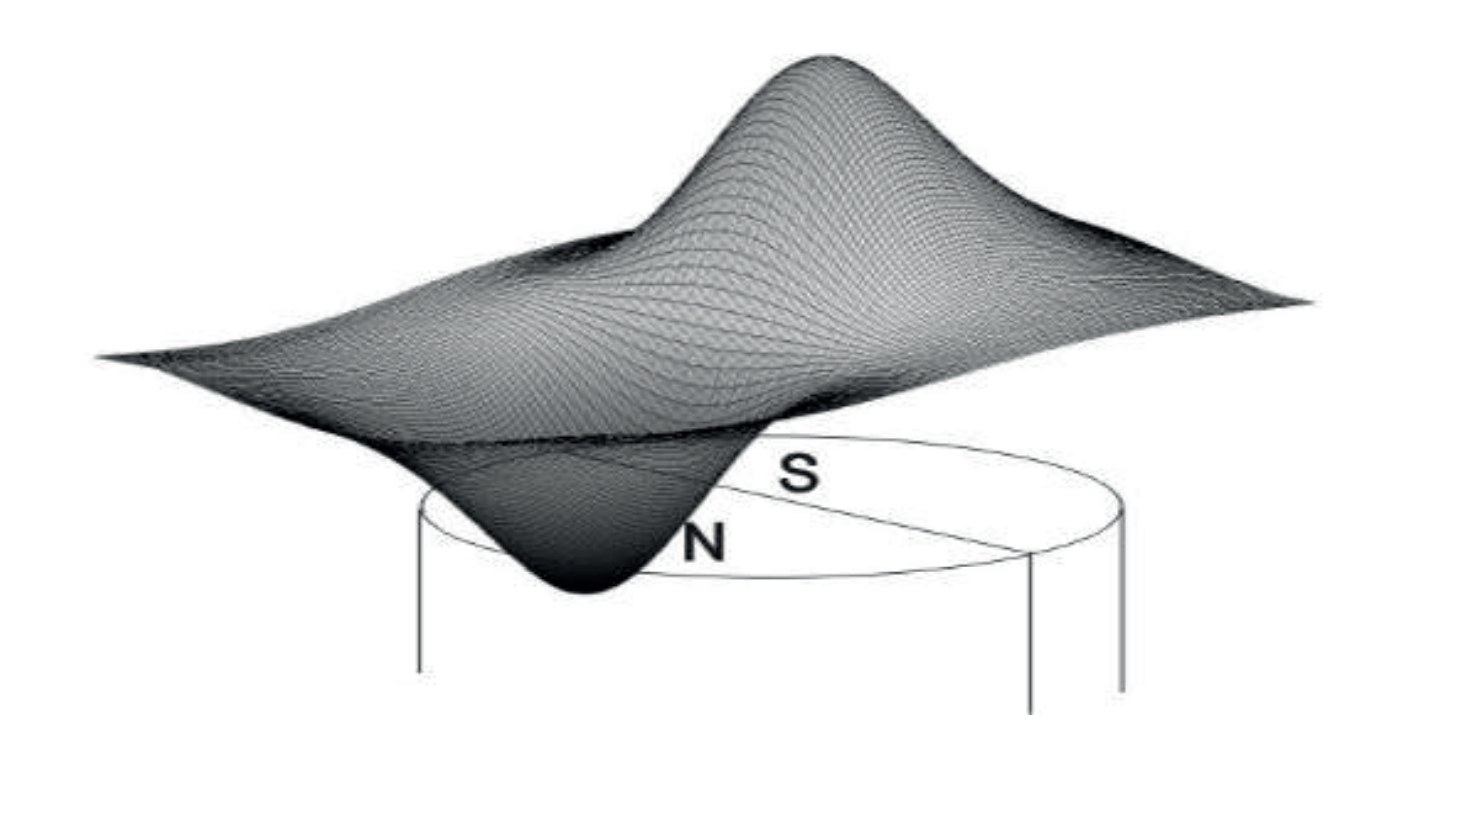
\includegraphics[width=0.75\columnwidth]{./Slike/magnetno_polje.jpg}
	\caption{z-komponenta vektorja gostote magnetnega polja nad cilindri"cnim magnetom citeAM8192}
	\label{fig:magnetno_polje}
\end{figure}


Potek z-komponente lahko izra"cunamo po Biot-Savartovim zakonom oz. numeri"cno se"stejemo prispevke posameznih del"ckov magneta. Tako dobimo vrednost celotnega vektorja gostote magnetnga polja v posamezni to"cki. Magnetno polje z komponente v okolici osi vrtenja magneta lahko aproksimiramo z ravnino

\begin{equation}
\label{equ:poljeB}
B_z(x,y)=k\cdot x.
\end{equation}

Tak"sna aproksimacija zadostuje za ocenitev poteka napake. S poznavanjem lokacije Hall-ove sonde, kar smo si ogledali v prej"snjem poglavju, sedaj dobimo potek pomerjene komponente gostote magnetnega polja. Aprokisirano polje je linearno odvisno od x komponente. Za la"zje razumevanje definirajmo konstanto $k$ enako 1.

\section{Postavitev Hall-ovih sond za zajem polja in pomerjeno polje v odvistnosti od ekscentri"cnosti}
%Sedaj si oglejmo, kako bi dolo"cili kot zasuka poljubne to"cke okoli izhodi"s"ca. Definirajmo kartezi"cni koordinatni sistem, in v njem poljubno to"cko $(x_0,y_0)$, ki ni v izhodi"s"cu(Slika \ref{fig:dolocitev_kota}).
%Za dolo"canje kota $\varphi$ je potrebno poznati poznati polo"zaj to"cke. Kot $\varphi$ dolo"cimo preko trigonometri"cne funkcije $\arctan$: $$\varphi=\arctan\frac{y_0}{x_0}$$
%
%
%
%\begin{figure}[h!]
%	\centering
%	\begin{tikzpicture}[scale=4]
%	\CaCS{0.75}{0}{0}
%	\draw [->,thick](0,0)--(-0.5,0.2855);
%	\draw (0.15,0) arc (0:150:0.15);
%	\node at (0.05,0.05){$\varphi$};
%%	\node at (-0.5,0.285) {\textbullet};
%	\node at (-0.32,0.35) {($x_0$,$y_0$)};
%	\end{tikzpicture}
%	\caption{Slika za pomo"c pri dolo"canju kota}
%	\label{fig:dolocitev_kota}
%\end{figure}
%
%
%Za dolo"citev kota $\varphi$  je dovolj poznati "ze projekciji vektorja na koordinatni osi(slika \ref{fig:dolocitev_kota_2}),
%
%\begin{figure}[h!]
%	\centering
%	\begin{tikzpicture}[scale=4]
%	\CaCS{0.75}{0}{0}
%	\draw [->,thick](0,0)--(-0.5,0.2855);
%	\draw (0.15,0) arc (0:150:0.15);
%	\node at (0.05,0.05){$\varphi$};
%	\draw [dashed] (-0.5,0.2855)--(-0.5,0);
%	\draw [dashed] (-0.5,0.2855)--(0,0.2855);
%	%	\node at (-0.5,0.285) {\textbullet};
%%	\node at (-0.32,0.35) {($x_0$,$y_0$)};
%	\node at(-0.5,-0.1){$x_0$} ;
%	\node at(0.1,0.2855){$y_0$};
%	\end{tikzpicture}
%	\caption{Slika za pomo"c pri dolo"canju kota}
%	\label{fig:dolocitev_kota_2}
%\end{figure}
%
%
%"Ce poznamo projekciji to"cke na koordinatni osi, je to zadosten pogoj za dolo"citev kota $\varphi$.
%Projekcijo lahko pridobimo "ce opazujemo projekciji polo"zaja to"cke v koordinatnih oseh.
%
%Sedaj si predstavljajmo da ta poljubna to"cka predstavlja enega od polov magneta. Za poznavanje zasuka pola magneta, je dovolj od"citanje polja na koordinatnih oseh. Hall-ovi sondi ne smeti biti postavljeni na isto koordinatno os. Ni nujno da sta sondi postavljeni pravokotno druga na drugo, si pa s tem prihranimo korak v katerem bi bilo potrebno izra"cunati projekcijo na pravokotni koordinatni osi.
%
%Iz zgornjega razmisleka lahko sedaj smiselno postavimo Hall-ovi sondi v koordinatni sistem. Najprimerneje ju je postaviti na koordinatni osi (Slika \ref{fig:zacetna_postavitev_sond}). Sondi postavimo na enako razdaljo od izhodi"s"ca $r_0$. Tako bo zajem poteka polja ob rotaciji magneta enak, le fazno zamaknjeno.


Za izra"cun kota potrebujem poznati polje v vsaj dveh to"ckah nad magnetom. Da si ena"cbe olaj"samo postavimo 2 Hall-ovi sondi na koordinatni osi, oddaljeni od izhodi"s"ca za $r_0$.

\begin{figure}[h!]
	\centering
	\begin{tikzpicture}[scale=1]
	\CaCS{3}{0}{0}
	\senzorja{0}{0}{0}{}
%	\magnet {0} {0} {10}{ }{0}
	\node at (2.0,-0.5){$\mathrm{H}_1(r_0,0)$};
	\node at (-1,2.3){$\mathrm{H}_2(0, r_0)$};
	\end{tikzpicture}
	\caption{Za"cetna postavitev Hallovih sond}
	\label{fig:zacetna_postavitev_sond}
\end{figure}

S poznavanjem lociranja sonde glede na magnet (\ref{equ:rotacija_hall_koncna}), funkcije polja (\ref{equ:poljeB}) ter za"cetne pozicije Hall-ovih sond lahko dolo"cimo potek polja sonde.

\begin{equation}\label{equ:Bx_splosna}
cos=B_{H_1}(\theta,r_0,\Delta x_s, \Delta y_s, \Delta x_d)= r_0 \cos\theta +\Delta x_s \cos\theta +\Delta y_s \sin\theta -\Delta x_d
\end{equation}
\begin{equation}\label{equ:By_splosna}
sin=B_{H_2}(\theta,r_0,\Delta x_s, \Delta y_s, \Delta x_d)= r_0 \sin\theta +\Delta x_s \cos\theta +\Delta y_s \sin\theta-\Delta x_d
\end{equation}

Zajeta signala bom od tu naprej imenoval sinus ($sin$) in cosinu ($cos$), ker je to njuna osnovna oblika.



\subsection{Sprememba magnetnega polja zaradi ekscentri"cnosti}

Oglejmo si primer kak"sno polje zajameti Hall-ovi sondi, ko ekscentri"cnosti ni. $sin$ in $cos$ izraza se poenostavita in dobimo poteka v obliki sinusa ter kosinusa z enako amplitudo (Slika \ref{./Napake/sincos_00}).

\slikaeps{Poteka $sin$ in $cos$ brez ekscentri"cnosti pri $r_0 = 1$ mm}{./Napake/sincos_00}
\newpage
Upo"stevajmo sedaj le stati"cni ekscentri"cnosti $\Delta x_s$ in $\Delta y_s$. $\Delta x_d$ postavimo na 0.   Ena"cbi (\ref{equ:Bx_splosna}) in (\ref{equ:By_splosna}) lahko preuredimo v izraza:


\begin{equation}
\label{equ:Bx_stat}
cos(\theta,r_0,\Delta x_s, \Delta y_s)= \sqrt{(r_0+\Delta x_s)^2+\Delta y_s^2}\cos(\theta -\arctan \frac{\Delta y_s}{r_0+\Delta x_s})
\end{equation}
\begin{equation}\label{equ:By_stat}
sin(\theta,r_0,\Delta x_s, \Delta y_s)= \sqrt{\Delta x_s^2+(r_0+\Delta y_s)^2} \sin(\theta +\arctan \frac{\Delta x_s}{r_0+\Delta y_s})
\end{equation}

Iz njiju vidimo spremenjena poteka. Signaloma se je spremenila amplituda in fazni zamik (Slika \ref{./Napake/sincos_xs}).

\slikaeps{Poteka $sin$ in $cos$ pri $r_0 = 1$ mm in upo"stevanjem 0,1 mm stati"cni ekscentri"cnosti v x-osi }{./Napake/sincos_xs}
\newpage
Postavimo sedaj vrednosti $\Delta x_s$ in $\Delta_ys$ na 0, $\Delta x_d$ predpostavimo da ni 0.
\begin{equation}
\label{equ:Bx_din}
cos(\theta,r_0,\Delta x_s, \Delta y_s, \Delta x_d)= r_0 \cos\theta-\Delta x_d
\end{equation}
\begin{equation}
\label{equ:By_din}
sin(\theta,r_0,\Delta x_s, \Delta y_s, \Delta x_d)= r_0 \sin\theta-\Delta x_d
\end{equation}
Polji obdr"zita enako amplitudo ter fazo, vendar dobita enosmerno komponento (Slika \ref{./Napake/sincos_xd}).
\slikaeps{Poteka $sin$ in $cos$ pri $r_0 = 1$ mm in upo"stevanjem 0,1 dinami"cne ekscentri"cnosti v x-osi}{./Napake/sincos_xd}\newpage
\section{Premik senzorja v z smeri}

Poglejmo si "se kako vpliva sprememba premikanja senzorja v z smeri.
Pri magnetnem polju aprokismiranem z ravnino (\ref{equ:lin_polje}), se gostota magnetnega polja pri obeh sondah spreminja enako. To se v ena"cbah odra"za le kot dodaten faktor. Upo"stevajmo spremembo polja zaradi premika senzorja po z osi. Zajeti polji imata naslednji potek:


\begin{equation}\label{equ:Bx_z}
cos=k_z( r_0 \cos\theta +\Delta x_s \cos\theta +\Delta y_s \sin\theta -\Delta x_d)
\end{equation}
\begin{equation}\label{equ:By_z}
sin=k_z( r_0 \sin\theta +\Delta x_s \cos\theta +\Delta y_s \sin\theta-\Delta x_d)
\end{equation}

Z vstavitvijo formul v $\arctan$ se faktor $k_z$ nahaj tako v "stevcu kot imenovalcu ter se lahko okraj"sa. Naj "se  enkrat poudarim, da to velja le za polje aproksimirano z ravnino.



\chapter{Vpliv deformacije signala sinus in cosinus na izhodno napako}

Da si lažje predstavljamo, kako se bo napaka odražala v obliki digitalnega izhoda, si oglejmo posamezno deformacijo signalov sinus in cosinus. Deformacija sinusa in cosinusa zaradi nepravilne montaže, vpliva le na enosmerno komponento, amplitudo in fazni kot med signaloma.

Ogledali si bomo kako vplivajo na izračunan kot, različne amplitude signalov sinus in cosinus, neortogonalost oz. fazni zamik sinusa in kosinusa različen od $90^\circ$. Ogledali si bomo tudi pojav enosmernih komponenet v sinusu in cosinusu, in za konec še vpliv višjih harmonikov, ki niso posledica nepravilne montaže, vendar je prav da jih omenim.

Za izračun kota se uporablja funkcijo atan2(); za izhodno vrednost kota v radianih oz. atan2d(); za vrednost v stopinjah \cite{atan2Matlab}\cite{atan2dMatlab}. Različne literature (citiraj iz clanaka od rls) opisujejo napake zaradi popačitve signalov sin cos. Napaka je izražena v obliki enosmerne komponente ter prvega oz drugega harmonika, kateri od primera do primera najbolj izstopa. V nadaljeevanju bom prikazal kako popačen signal kot vhod v funkcijo atan2(); vpliva na napako ter kako se odraža tudi na visjih harmonikih napake. Za majhne popačenja signalov, literatura nakazuje na linearno naraščanje napake, vendar predvidevam, da bo napaka z večjo deformacijo naraščala eksponentno.

Na tej točki je prav da definiram še napako pomejrenega kota $\varepsilon$, ki predstavlja razliko med merjenim in referenčnim kotom.

\begin{equation}
\varepsilon = \varphi - \mathrm{atan2}(\sin{\theta},\cos{\theta})
\end{equation}


\section{Različne amplitude}

Vzemimo signal sinus z amplitudo $A_{sin}$ in signal cosinus z amplitude $A_{cos}$. Vstavimo signala v funkcijo $atan2$.

Opazimo, da lahhko razmerje amplitud nadomestimo s koeficientom $k$. Kot, ki bo izhodna funkcija lahko nadosmetimo s:
\begin{equation}
\varphi =  \mathrm{atan2}(A_{sin} \sin{\theta}, A_{cos} \cos{\theta}) = \mathrm{atan2}(k \sin{\theta},\cos{\theta})
\end{equation}

k limitirajmo v neskončnost:
\begin{equation}
\lim_{k \rightarrow \infty} \mathrm{atan2}(k \sin{\theta},\cos{\theta})
\end{equation}

\slikaeps{$\varepsilon$ ob limiti k v neskončnost }{./Napake/k_lim}

Kot $\varepsilon$, se bo ob limiti  izrazila v obliki , ki jo lahko izrazimo z vrsto \cite{fourierova_vrsta}:

\begin{equation}
\varepsilon = \frac{180}{\pi}\sum_{n=1}^{\infty}\frac{1}{n} \sin 2 n \theta
\end{equation}

Nato sem izračunal napaka pri različnih k in naredil fft napake $\varepsilon$ \cite{matlab_fft}.

Harmonike napake sem aproksimiral z racionalno funkcijo in končna napaka za katerikoli k se je izrazila z vrsto:

\begin{equation}
\label{vrsta_k}
\varepsilon_p =\frac{180}{\pi}\sum_{n=1}^{\infty}\frac{1}{n}(\frac{k-1}{k+1})^n \sin 2 n \theta
\end{equation}

\slikaeps{$\varepsilon$ pri k=1.1 }{./Napake/napaka_amp11}
\slikaeps{Razlika med napako izračunano s funkcijo atan2 in izračnunano napako z vrsto po (\ref{vrsta_k}) pri k= 1.1 }{./Napake/razlika_amp11}
\newpage
\section{Različne enosmerne komponente}

Enosmerna komponenta se lahko pojavi tako v sinusu, cosinusu ali v obeh. V naslednjih podpoglavjih bom prikazal kako se napaka spreminja glede na enosmerno komponeno le v enem od signalov in nakoncu kako se napaka izrazi, če imate oba signala enake enosmerne komponente.

\subsection{Enosmerna komponenta sinusa}

Poglejmo kako se bo izrazala napaka $\varepsilon$ v naslednjem izrazu:
\begin{equation}
\varphi = \mathrm{atan2}(\sin{\theta} + b_0,\cos{\theta})
\end{equation}

Postopajmo kot v prejčnjem poglavju in limitirajmo $b_0$ v neskončnost:

\begin{equation}
\lim_{b_0 \rightarrow \infty} \mathrm{atan2}(\sin{\theta}+b_0,\cos{\theta})
\end{equation}

\slikaeps{$\varepsilon$ ob limiti $b_0$ v neskončnost }{./Napake/lim_sin}

Napaka se izrazi v obliki:

\begin{equation}
\varepsilon = \frac{180}{\pi}\sum_{n=1}^{\infty}\frac{2}{n} \sin (n \theta + 90 n)
\end{equation}


Tudi tu naredimo fft napake pri različnih enosmernih komponentah. Napako lahko opišemo z naslednjo enačbo:

\begin{equation}
\label{vrsta_sinoff}
\varepsilon_p=
\begin{cases}
\frac{180}{\pi}\sum_{n=1}^{\infty}\frac{2-|b_0|^{-n}}{n} \sin (n \theta -  90 n), & b_0\leq -1 \\
\frac{180}{\pi}\sum_{n=1}^{\infty}\frac{b_0^n}{n} \sin (n \theta + 90 n), & |b_0|\leq 1 \\
\frac{180}{\pi}\sum_{n=1}^{\infty}\frac{2-b_0^{-n}}{n} \sin (n \theta + 90 n), & b_0\geq 1
\end{cases}
\end{equation}

\slikaeps{$\varepsilon$ pri $b_0=$ 0,1 }{./Napake/napaka_sin01}
\slikaeps{Razlika med napako izračunano s funkcijo atan2 in izračnunano napako z vrsto po (\ref{vrsta_sinoff}) pri $b_0=$ 0,1 in $n < 20$}{./Napake/razlika_sin01}




\subsection{Enosmerna komponenta cosinusa}

Sedaj poglejom napako pri enosmerni komponenti cosinusa
\begin{equation}
\varphi = \mathrm{atan2}(\sin{\theta},\cos{\theta} + a_0)
\end{equation}

Postopajmo kot v prejčnjem poglavju in limitirajmo $a_0$ v neskončnost:

\begin{equation}
\lim_{a_0 \rightarrow \infty} \mathrm{atan2}(\sin{\theta},\cos{\theta} + a_0)
\end{equation}
\slikaeps{$\varepsilon$ ob limiti $a_0$ v neskončnost }{./Napake/lim_cos}

Napaka se izrazi v obliki:

\begin{equation}
\varepsilon = \frac{180}{\pi}\sum_{n=1}^{\infty}\frac{2}{n} \sin (n \theta+ 90 n)
\end{equation}


Tudi tu naredimo fft napake pri različnih enosmernih komponentah. Napako lahko opišemo z naslednjo enačbo:

\begin{equation}
\label{vrsta_cosoff}
\varepsilon_p=
\begin{cases}
\frac{180}{\pi}\sum_{n=1}^{\infty}(-1)^n\frac{2-|a_0|^{-n}}{n} \sin (n \theta ), & a_0\leq -1 \\
\frac{180}{\pi}\sum_{n=1}^{\infty}(-1)^n\frac{a_0^n}{n} \sin (n \theta ), & |a_0|\leq 1 \\
\frac{180}{\pi}\sum_{n=1}^{\infty}(-1)^n\frac{2-a_0^{-n}}{n} \sin (n \theta ), & a_0\geq 1
\end{cases}
\end{equation}

\slikaeps{$\varepsilon$ pri $a_=0$ 0,1 }{./Napake/napaka_cos01}
\slikaeps{Razlika med napako izračunano s funkcijo atan2 in izračnunano napako z vrsto po (\ref{vrsta_cosoff}) pri $a_0=$ 0,1 in $n < 20$ }{./Napake/razlika_cos01}

\newpage
\subsection{Enosmerna komponenta pri obeh signalih}
\label{2_offseta}
Oglejmo si še napako, če imate oba signala, sinus in cosinus, enako enosmerno komponento.


\begin{equation}
\varphi = \mathrm{atan2}(\sin{\theta} + c_0,\cos{\theta} + c_0)
\end{equation}

Limitirajmo:

\begin{equation}
\lim_{c_0 \rightarrow \infty} \mathrm{atan2}(\sin{\theta} + c_0,\cos{\theta}+ c_0) 
\end{equation}

\slikaeps{$\varepsilon$ ob limiti $c_0$ v neskončnost }{./Napake/lim_sincos}

in napako $\varepsilon$ zapišemo kot:

\begin{equation}
\varepsilon = \frac{180}{\pi}\sum_{n=1}^{\infty}\frac{2}{n} \sin (n \theta- 90 n)
\end{equation}


Z enakimi postopki kot zgoraj sem tudi tu določil potek napake.


\begin{equation}
\label{vrsta_sincosoff}
\varepsilon_p=
\begin{cases}
\frac{180}{\pi}\sum_{n=1}^{\infty}\frac{2-|\sqrt{2}c_0|^{-n}}{n} \sin (n \theta + 90 n), & c_0\leq -\frac{\sqrt{2}}{2} \\
\frac{180}{\pi}\sum_{n=1}^{\infty}\frac{(\sqrt{2}c_0)^n}{n} \sin (n \theta - 90 n), & |c_0|\leq \frac{\sqrt{2}}{2} \\
\frac{180}{\pi}\sum_{n=1}^{\infty}\frac{2-(\sqrt{2}c_0)^{-n}}{n} \sin (n \theta - 90 n), & c_0\geq \frac{\sqrt{2}}{2}
\end{cases}
\end{equation}

\slikaeps{$\varepsilon$ pri $c_0=$ 0,1 }{./Napake/napaka_sincos01}
\slikaeps{Razlika med napako izračunano s funkcijo atan2 in izračnunano napako z vrsto po (\ref{vrsta_sincosoff}) pri $c_0=$ 0,1 in $n < 20$}{./Napake/razlika_sincos01}




\section{Neorotogonalnost signalov}

Napaka se pojavi lahko tudi, če signala sinus in cosinus nista zamaknjena za točno $90^\circ$. Z enakim postopkom kot v prejšnjih poglavjih, bom tudi tu, določil napako z vrsto, za vsak zamaknjen signal posebaj.

\subsection{Fazni zamik sinusa}

Poglejmo najprej zamaknjen sinusni signal. Tudi tu napravimo limito vendar le do $90^\circ$, saj se siganl kasneje začne ponavljati.



\begin{equation}
\lim_{\varphi_{sin} \rightarrow 90} \mathrm{atan2}(\sin{\theta+\varphi_{sin}} ,\cos{\theta}) 
\end{equation}


\slikaeps{$\varepsilon$ pri  $\varphi_{sin}= 90^\circ$  }{./Napake/lim_sinfaza}

Napaka se izrazi v vrsti:

\begin{equation}
\varepsilon = 45^\circ - \frac{180}{\pi}\sum_{n=1}^{\infty}\frac{1}{n} \sin (2n \theta)
\end{equation}


Napravil sem izračune napake pri različnih $\varphi_{sin}$, naredil fft signala in pogledal odvistnost amplitude harmonika od $\varphi_{sin}$. Harmonike sem lahko aprokismiral z višjimi potencami funkcije tangens, ter dobil končno enačbo.


\begin{equation}
\label{vrsta_faza_sin}
\varepsilon_p = \frac{\varphi_{sin}}{2} + \frac{180}{\pi}\sum_{n=1}^{\infty}\frac{1}{n} \mathrm{tan}(\frac{\varphi_{sin}}{2})^n \sin (2n \theta+90 n +n \varphi_{sin})
\end{equation}


\slikaeps{$\varepsilon$ pri $\varphi_{sin} = 1^\circ$ }{./Napake/napaka_fazasin1}
\slikaeps{Razlika med napako izračunano s funkcijo atan2 in izračnunano napako z vrsto po (\ref{vrsta_faza_sin}) pri  $\varphi_{sin} = 1^\circ$ in $n < 20$}{./Napake/razlika_fazasin1}


\subsection{Fazni zamik cosinusa}

Enako posotopamo tudi pri faznem zamiku cosinusa.



\begin{equation}
\lim_{\varphi_{cos} \rightarrow 90} \mathrm{atan2}(\sin{\theta+\varphi_{cos}} ,\cos{\theta}) 
\end{equation}


\slikaeps{$\varepsilon$ pri  $\varphi_{cos}= 90^\circ$  }{./Napake/lim_cosfaza}

Napaka se izrazi v vrsti:

\begin{equation}
\varepsilon = 45^\circ + \frac{180}{\pi}\sum_{n=1}^{\infty}\frac{1}{n} \sin (2n \theta)
\end{equation}


Ponovil pri različnih $\varphi_{cos}$, naredil fft, aproksimiral posamezni harmonik napake in dobil izraz:


\begin{equation}
\label{vrsta_faza_sin}
\varepsilon_p = \frac{\varphi_{cos}}{2} + \frac{180}{\pi}\sum_{n=1}^{\infty}\frac{1}{n} \mathrm{tan}(\frac{\varphi_{cos}}{2})^n \sin (2n \theta- 90 n+n \varphi_{cos})
\end{equation}


\slikaeps{$\varepsilon$ pri $\varphi_{cos} = 1^\circ$ }{./Napake/napaka_fazacos1}
\slikaeps{Razlika med napako izračunano s funkcijo atan2 in izračnunano napako z vrsto po (\ref{vrsta_faza_sin}) pri  $\varphi_{cos} = 1^\circ$ in $n < 20$}{./Napake/razlika_fazacos1}


\newpage
\section{Potek napake pri statični ekscentričnosti v smeri x}

V zgornjih poglavjih smo spoznali, kakšne oblike je napaka pri določeni deformaciji analognega signala.
Zgornji poteki napake veljajo le za eno vrsto deformacije, njihovih odvistnosti nisem raziskal.

Sedaj se osredotočimo na potek napake ob izraženi statični ekscentričnosti v smeri x. Signala $sin$ in $cos$ imate naslednji potek:

\begin{eqnarray}
\label{xs_analit}
sin = r_0 \sin(\theta) + \Delta x_s \cos(\theta) \\
cos = r_0 \cos(\theta) + \Delta x_s \cos(\theta)
\end{eqnarray}

Kot $\varphi$ bomo pridobili s funkcijo atan2(). Zgornja izraza vstavimo v atan2() in ju delimo z $r_0$.
 
 \begin{equation}
 \varphi = \mathrm{atan2}(\sin(\theta) + \frac{\Delta x_s}{r_0} \cos(\theta),\cos(\theta) + \frac{\Delta x_s}{r_0} \cos(\theta))
 \end{equation}
 
 Napako sem izpelajal po enakih postopkih kot zgoraj.
 Napaka sem izrazil z vrsto:
 
 \begin{equation}
 \label{vrsta:xs}
 \varepsilon_p = \mathrm{atan}\frac{\Delta x _s}{\Delta x _s+2r_0}+\frac{180}{\pi} \sum_{n=1}^{\infty}\frac{1}{n} (\frac{\Delta x _s}{\sqrt{\Delta x _s^2+2 r_0 \Delta x _s+2r_0^2}})^n \sin (2n \theta+n (90+ \mathrm{ atan}(\frac{\Delta x _s+r_0}{r_0})))
 \end{equation}
 
 Pri čemer:
 $$\Delta x_s > -r_0$$
 
 Napaka se je izrazila z enosmerno komponento in drugim harmonikom, po pričakovanju. V enačbi (\ref{xs_analit}) vidimo, da nastopati v analognih signalih razilčni amplitudi in fazna zamika. Napaka  je bila pričakovana.
 
 
 
 \section{Potek napake pri statični ekscentričnosti v smeri y}
 
 Postopek enako ponovimo za ekscentričnost v y smeri. Pričakujem, da se bo napaka izrazila podobno kot, pri ekscentričnosti v x smeri.
 
 Izpeljal sem napako z vrsto in rezultat je: 
 
  \begin{equation}
   \label{vrsta:ys}
 \varepsilon_p = \mathrm{atan}\frac{-\Delta y _s}{\Delta y _s+2r_0}+\frac{180}{\pi} \sum_{n=1}^{\infty}\frac{1}{n} (\frac{\Delta y _s}{\sqrt{\Delta y _s^2+2 r_0 \Delta y _s+2r_0^2}})^n \sin (2n \theta+n (90+ \mathrm{ atan}(\frac{\Delta y _s+r_0}{r_0})))
 \end{equation}

 Pri čemer:
$$\Delta y_s > -r_0$$

\section{Potek napake pri dinamični ekscentričnosti v smeri x}

Analogna signala se izrazita z naslednjim potekom:

\begin{eqnarray}
sin = r_0 \sin(\theta) - \Delta x_d \\
cos = r_0 \cos(\theta) - \Delta x_d
\end{eqnarray}

Signala nas spomnita na poteka, ki smo ju obravnavali že v poglavju \ref{2_offseta}, zato bom tu napisal le rezultat. Razlikuje se le v predznaku.

\begin{equation}
\label{vrsta_xd}
\varepsilon_p=
\frac{180}{\pi}\sum_{n=1}^{\infty}\frac{1}{n}( \frac{-\sqrt{2}}{r_0}\Delta x_d)^n \sin (n \theta -  90 n)
\end{equation}


$$|\Delta x_d|\leq \frac{r_0}{\sqrt{2}}$$


V tem poglavju smo pogledali, poteke napake ob deformaciji analognih signalov. Ogledali smo si tudi, kako se bo napaka izrazila ob ekcentričnosti senzorja ter magneta. Za majhne odmike, je dovolj upoštevanje le prvega člena vrste, pri katerih lahko tudi predpostavimo linearno naraščanje napake. V nadaljevanju bom velikost harmonika v odvistnosti od povzročene ekscentričnosti aproksimiral s kubičnim polinomom, ter jih primerjal z izpeljavo v tem poglavju. Harmoniki katerih potek je npr racionalna funkcija (primer (\ref{vrsta:xs})), bom razvil v Taylorjevo vrsto do tretje stopnje, katero bom lahko primerjal s kubičnimi polinomi.
 









%\section{Analiti"cen potek napake posamezne ekscentri"cnosti}
%
%S poznavanjem potekov polja posamezne sonde sedaj s funkcijo $\arctan$ izra"cunamo kot.
%
%\begin{equation}
%\label{equ:izracun_kota_splosna}
%\varphi(\theta,\Delta x_s, \Delta y_s, \Delta x_d)=\arctan\frac{B_y}{B_x}=\arctan\frac{r_0 \sin\theta +\Delta x_s \cos\theta +\Delta y_s \sin\theta-\Delta x_d}{r_0 \cos\theta +\Delta x_s \cos\theta +\Delta y_s \sin\theta -\Delta x_d}
%\end{equation}
%
%
%
%
%Iz podanega izraza (\ref{equ:izracun_kota_splosna}) je te"zko sklepati, kak"sen bo potek pomerjenega kota.
%Na tem mestu definirajmo napako merjenega kota:
%\begin{equation}
%\varepsilon=\varphi-\theta
%\end{equation}
%
%Poglejmo si analiti"cen potek napake.  S spodaj opisanim postopkom se bomo izognili numeri"cnemu ra"cunanju funkcije $\arctan$.
%
%Signala $sin$ in $cos$ imata periodo $360^\circ$. Iz tega sledi, da bo tudi $\varepsilon$ imel periodo $360^\circ $. Pri"cakujem, da bo potek napake $\varepsilon$ v obliki :
%\begin{equation}
%\label{equ:nastavek}
%\varepsilon=A_0+A_1 \cos \theta +B_1 \sin \theta+A_2 \cos 2\theta +B_2 \sin 2\theta
%\end{equation}
%Tak nastavek sem vzel zaradi predvidene napake v podatkovnih listih citeAM8192.
%Za pribli"zek napake izraz  (\ref{equ:izracun_kota_splosna}) razvijmo v Taylorjevo vrsto po kotu $\theta$. V Taylorjevo vrsto razvjemo tudi nastavek pri"cakovanega poteka. Zaradi aproksimacije poteka merjenega kota se zadovoljimo z razvojem do petega reda. Za poenostavitev se bom ekscentri"cnosti lotil posamezno. V naslednjih podpoglavjih bom prikazal analiti"cne rezultate posameznega harmonika. Izpeljavo bom le teoreti"cno opisal.
%
%Oba izraza (\ref{equ:izracun_kota_splosna} in \ref{equ:nastavek} )razvijem do petega reda Taylorjeve vrste  po kotu $\theta$. Z zdru"zitvijo posameznih potenc $\theta$, pridobimo sistem petih en"cb s petimi neznankami. S tem pridobim neznane faktorje $A_0$, $A_1$, $A_2$, $B_1$ in $B_2$. S poznavanjem teh faktorjev lahko ocenimo ka"skni bodo poteki posameznih harmonikov, ob posameznih ekscentri"cnostih. Te rezultate Taylorjeve vrste lahko upo"stevam le v okolici ni"cle. Izrazi so izpeljani za stati"cni ekscentri"cnosti ter dinami"cno ekscentri"cnost v smeri x. Potekov dinami"cne ekscentri"cnosti v smeri y ni, saj ta ne nastopa v izrazu (\ref{equ:izracun_kota_splosna}).
%\subsection{Aproksimacija pomerjenega kota ob stati"cni ekscentri"cnosti x}
%V izrazu (\ref{equ:izracun_kota_splosna}) upo"stevamo le stati"cno ekscentri"cnost $\Delta x_s$.
%\begin{equation}
%\label{equ:izracun_kota_xs}
%\varphi=\arctan \frac{r_0 \sin\theta +\Delta x_s \cos\theta}{r_0 \cos\theta +\Delta x_s \cos\theta}
%\end{equation}
%Z aproksimacijo po izrazu (\ref{equ:nastavek}) pridobimo koeficiente posameznega harmonika
%
%\begin{eqnarray}
%&A_0=\frac{-90 r_0^2  \Delta y_s (r_0^5+29 r_0^4 \Delta y_s+132 r_0^3  \Delta y_s^2+208 r_0 ^2  \Delta y_s^3+156 r_0  \Delta y_s^4+52 \Delta y_s^5)}{\pi (r_0^2+2 r_0 \Delta y_s+2 \Delta y_s^2)^4}+\arctan \frac{ \Delta y_s}{r_0+ \Delta y_s}\\
%&A_1=\frac{2280 r_0^2  \Delta y_s^2(r_0^4+5 r_0^3  \Delta y_s+8 r_0^2  \Delta y_s^2+6 r_0  \Delta y_s^3+2 \Delta y_s^4)}{\pi(r_0^2+2 r_0 \Delta y_s+2 \Delta y_s^2)^4}\\
%&B_1=-\frac{240 \Delta y_s^3(7r_0^3+18 r_0^2  \Delta y_s+18 r_0^2  \Delta y_s+18 r_0  \Delta y_s^2+8 \Delta y_s^3)}{\pi(r_0^2+2 r_0 \Delta y_s+2 \Delta y_s^2)^3}\\
%&A_2=\frac{90 r_0^2  \Delta y_s (r_0^5-3 r_0^4 \Delta y_s-28 r_0^3  \Delta y_s^2-48r_0 ^2  \Delta y_s^3-36 r_0  \Delta y_s^4-12 \Delta y_s^5)}{\pi(r_0^2+2 r_0 \Delta y_s+2 \Delta y_s^2)^4}\\
%&B_2=\frac{30 \Delta y_s (-3r_0^5-18 r_0^4 \Delta y_s-20 r_0^3  \Delta y_s^2 +12 r_0  \Delta y_s^4+8 \Delta y_s^5)}{\pi(r_0^2+2 r_0 \Delta y_s+2 \Delta y_s^2)^3}\\
%\end{eqnarray}
%Oglejmo si sliko potekov posameznih harmonikov.
%\slikaeps{Poteki amplitud prvega in drugega harmonika ter enosmerne komponente ob spreminjanju stati"cne ekscentri"cnosti v x-osi}{potek_analitika_xs}
%Iz rezultatov lahko pri"cakujemo nara"s"canje drugega harmonika ter nara"s"canje enosmerne komponete.
%\subsection{Aproksimacija pomerjenega kota ob stati"cni ekscentri"cnosti y}
%V izrazu (\ref{equ:izracun_kota_splosna}) upo"stevamo le stati"cno ekscentri"cnost $\Delta y_s$.
%\begin{equation}
%\label{equ:izracun_kota_ys}
%\varphi=\arctan \frac{r_0 \sin\theta +\Delta y_s \sin\theta}{r_0 \cos\theta +\Delta y_s \sin\theta}
%\end{equation}
%Z aproksimacijo po izrazu (\ref{equ:nastavek}) pridobimo koeficiente posameznega harmonika
%\begin{eqnarray}
%&A_0=\frac{-90 y_s (r_0^2-23r_0 y_s-24y _s^2)}{\pi r_0^3}\\
%&A_1=\frac{-1690 y_s^2(r_0+y_s)}{\pi r_0^3}\\
%&A_2=\frac{90 y_s(r_0^2+9r_0y_s+8y_s^2)}{\pi r_0^3}\\
%&B_1=\frac{240 y_s^3}{\pi r_0^3}\\
%&B_2=\frac{30 (3 r_0^2y_s-4 y_s^3)}{\pi r_0^3}
%\end{eqnarray}
%Oglejmo si sliko potekov posameznih harmonikov.
%\slikaeps{Poteki amplitud prvega in drugega harmonika ter enosmerne komponente ob spreminjanju stati"cne ekscentri"cnosti v y-osi}{potek_analitika_ys}
%Iz grafa je razvidno, da do enosmerna komponenta upadala, drugi harmonik bo najbolj izrazit.
%\subsection{Aproksimacija pomerjenega kota ob dinami"cni ekscentri"cnosti x}
%Izraz  (\ref{equ:izracun_kota_splosna}) kjer upo"stevamo le dinami"cno ekscentri"cnost se poenostavi v:
%\begin{eqnarray}
%&A_0=\frac{180(r_0 \Delta x_d(r_0^6-7r_0^5 \Delta x_d+18r_0^4 \Delta x_d^2-36r_0^2 \Delta x_d^4 +28r_0 \Delta x_d^5-8 \Delta x_d^6))}{\pi(r_0^2-2r_0 \Delta x_d+2 \Delta x_d^2)^4}-\arctan \frac{\Delta x_d}{r_0- \Delta x_d}\\
%&A_1=\frac{-180(r_0 \Delta x_d(r_0^6-8r_0^5 \Delta x_d+22r_0^4 \Delta x_d^2-44r_0^2 \Delta x_d^4 
%	+32r_0 \Delta x_d^5-8 \Delta x_d^6)}{\pi (r_0^2-2r_0 \Delta x_d+2 \Delta x_d^2)^4)}\\
%&A_2=\frac{-180(r_0^2 \Delta x_d^2 (r_0^4-4 r_0^3  \Delta x_d+8 r_0  \Delta x_d^3-4 
%	\Delta x_d^4)}{\pi (r_0^2-2 r_0  \Delta x_d+2  \Delta x_d^2)^4)}\\
%&B_1=\frac{60( \Delta x_d (3 r_0^5-18 r_0^4  \Delta x_d+64 r_0^3  \Delta x_d^2 -108 
%	r_0^2  \Delta x_d^3+84 r_0  \Delta x_d^4-32  \Delta x_d^5))}{\pi (r_0^2-2 r_0 
%	\Delta x_d+2  \Delta x_d^2)^3}\\
%&B_2=\frac{60 (2  \Delta x_d^3 (-4 r_0^3+9 r_0^2  \Delta x_d-6 r_0  \Delta x_d^2+2  \Delta x_d
%	^3))}{\pi(r_0^2-2 r_0  \Delta x_d+2  \Delta x_d^2)^3}
%\end{eqnarray}
%\slikaeps{Poteki amplitud prvega in drugega harmonika ter enosmerne komponente ob spreminjanju dinami"cne ekscentri"cnosti v x-osi}{potek_analitika_xd}
%S slike \ref{potek_analitika_xd} vidimo da bo izrazit le prvi harmonik, ki pri majhnih odmikih nara"s"ca linearno, kar je pri"cakovano po citeAM8192. 
%
%V tem poglavju smo si ogledali kak"sno magnetno polje ustvari magnet in kako ga Hall-ove sonde zaznavajo. magnetno polje smo aproksimirali z ravnino in si ogledali poteke napake.  Spoznali smo tudi kako se bo izra"zala napaka pri posamezni ekscentri"cnosti.
%
%
%
%
%
%
%
%
%












%
%
%
\chapter{Linearni model magnetnega polja}
\label{linearnimodel}

Za oceno napake, se lahko Z komponento magnetnega polja v okolici središča magneta, aproksimira z ravnino (slika \ref{polje_z_ravnino}).
Aproksimacija zadostuje za oceno napake. S poznavanjem lokacije sonde glede na magnet, se lahko izračuna merjena komponenta magnetnega polja. Aprokisimirano polje je linearno odvisno od x komponente (\ref{equ:poljeB1}).  Za lažje razumevanje bo $k$ enak $1\frac{\mathrm{mT}}{\mathrm{mm}}$.
\begin{equation}
\label{equ:lin_polje}
B_z(x,y)=k\cdot x.
\end{equation}
\begin{figure}[ht]
	\centering
	\includegraphics[width=0.6 \columnwidth]{./Slike/polje_z_ravnino.eps}
	\caption{Oblika Z komponente gostote magnetnega polja nad magnetom in aproksimirano ravnino v središču magneta}
	\label{polje_z_ravnino}
\end{figure}
\newpage

Simulacijski model sestavljajo 4 Hallove sonde enakomerno razporejene po krožnici z radijem $r_0$ (slika \ref{lin_simul}). Lokacija predstavlja začetno lego Hallovih sond. 
Ob zasuku magneta, se sonde relativno gibljejo na magnet v nasprotni smeri kot se vrti magnet. 
\begin{figure}[!ht]
	\centering
	\begin{tikzpicture}
	\magnet {0} {0} {0}{ }{1};
	\hall {1}{0} {0};
	\hall {0}{1} {0};
	\hall {-1}{0} {0};
	\hall {0}{-1} {0};
	\draw [dotted](0,1)--(0,0)--(1,0);
	\draw [dotted] (0,0) circle [radius=1];
	\draw [<->]	(0,0) -- (0.866,-0.5) node [black,midway,yshift= -0.2cm] 
	{\footnotesize $r_0$};
	\draw[<-](1.2,0.3)--(2.1,1)node[anchor = west]{$H_1(r_0,0)$};
	\draw[<-](-0.25,1.1)--(-1,2.2)node[anchor = south]{$H_2(0,r_0)$};
	\draw[<-](-1.2,0.3)--(-2.1,1)node[anchor = east]{$H_3(-r_0,0)$};
	\draw[<-](-0.25,-1.1)--(-1,-2.2)node[anchor = north]{$H_4(0,-r_0)$};
	\end{tikzpicture}
	\caption{Shema simulacijskega modela}
	\label{lin_simul}
\end{figure}

Z upoštevanjem vplivov ekscentričnosti iz izraza (\ref{equ:rotacija_hall_koncna}) in enačbe za izračun Z-komponente gostote magnetnega pretoka (\ref{equ:lin_polje}) se izrazi potek polja, ki ga pomeri posamezna sonda ob vrtenju.
\begin{eqnarray}
\label{equ:lin_potek_sin}
B_{H_1}(\theta, r_0, \Delta x_s, \Delta y_s, \Delta x_d, \Delta y_d)=  r_0 \cos \theta + \Delta x_s \cos \theta+ \Delta y_s \sin \theta -\Delta x_d\\
\label{equ:lin_potek_cos}
B_{H_2}(\theta, r_0, \Delta x_s, \Delta y_s, \Delta x_d, \Delta y_d)= r_0 \sin \theta + \Delta x_s \cos \theta+ \Delta y_s \sin \theta -\Delta x_d\\
B_{H_3}(\theta, r_0, \Delta x_s, \Delta y_s, \Delta x_d, \Delta y_d)=  -r_0 \cos \theta + \Delta x_s \cos \theta+ \Delta y_s \sin \theta -\Delta x_d\\
\label{equ:lin_potek_zadnja}
B_{H_4}(\theta, r_0, \Delta x_s, \Delta y_s, \Delta x_d, \Delta y_d)=-r_0 \sin \theta + \Delta x_s \cos \theta+ \Delta y_s \sin \theta -\Delta x_d
\end{eqnarray}
Z odštevanjem signalov nasprotni ležečih sond se pridobi signala  $B_{sin}$ in $B_{cos}$.
\begin{eqnarray}
B_{sin}=  B_{H_1} - B_{H_3} = 2 r_0 \sin \theta \\
B_{cos}=  B_{H_2} - B_{H_4}=  2 r_0 \cos \theta
\end{eqnarray}

Z diferencialnim odčitavenjem signalov  $B_{sin}$ in $B_{cos}$, se popačanje signalov zaradi napačne montaže izniči. Iz tega sledi zaključek, da pri linearni apoksimaciji Z-komponente gostote magnetnega pretoka napačna montaža ne vpliva na napako.

Kljub temu so bile opravljene simulacije na poenostavljenem modelu, uporabi le dveh sond
 ($B_{sin}=B_{H_1}$ in $B_{cos}=B_{H_2}$). Na ta način je lahko bila analizirana napaka.
 
 Koeficient $k$, ki je v simulacijah enak $1 \frac{\mathrm{ mT}}{\mathrm{ mm}}$, bi bil lahko tudi poljuben.
 Izraza $B_{sin}$ in $B_{cos}$ bi bila tako le množena s koeficientom $k$. Za izračun kota, se znotraj funkcije $atan2()$ izračuna kvocient med $B_{sin}$ in $B_{cos}$. Ker se $k$ pojavi tako v števcu in imenovaluc, se izniči. Koeficient $k$ na napako kota ne vpliva.

V tem poglavju so predstavljeni rezultati simulacij z upoštevanjem dveh Hall-ovih sond in uporabo linearno aprokismirane Z-komponente gostote magnetnega pretoka.
Prikazan je potek napake pri različnih izmikih, ter potek amplitud posameznih harmonikov napake v odvisnosti od ekscentričnosti.
Hall-ovi sondi sta postavljeni na krožnico z radijem 1,5 mm \cite{AM8192}.
\section{Brez ekscentričnosti}
Signala $B_{sin}$ in $B_{cos}$ pomerjena v stanju brez ekscentričnosti imata enaki amplitudi in sta fazno zamaknjena za $90^{\circ}$ ter brez enosmernih komponent. Napaka $\varepsilon$, ki se pojavi pri izračunu je le numerična napaka funkcije atan2d(); (Slika \ref{./LIN/yd_napaka}). Numerična napaka je proti pričakovani napaki zaradi ekscnetričnosti zanemarljiva.
\slikaeps{$B_{sin}$ in $B_{cos}$ pri simulacijah z linearnim magnetnim poljem brez ekscentričnosti}{./LIN/yd_sincos}
\slikaeps{Napaka $\varepsilon$ pri simulacijah z linearnim magnetnim poljem brez ekscentričnosti}{./LIN/yd_napaka}
\newpage
\section{Simulacija statične ekscentričnosti v smeri x-osi}
Izraza (\ref{equ:lin_potek_sin}) in (\ref{equ:lin_potek_cos}), se lahko preuredi:
\begin{eqnarray}
\label{equ:linearna_atan_sin}
B_{sin}= \sqrt{(r_0+\Delta y_s)^2+\Delta x_s^2} \sin(\theta+  \mathrm{ atan} \frac{\Delta x_s}{\Delta y_s +r_0})-\Delta x_d\\
\label{equ:linearna_atan_cos}
B_{cos}= \sqrt{(r_0+\Delta x_s)^2+\Delta y_s^2} \cos(\theta-  \mathrm{ atan} \frac{\Delta y_s}{\Delta x_s +r_0}) -\Delta x_d.
\end{eqnarray}

Ob upoštevanju le statične ekscentričnosti v smeri x se iz (\ref{equ:linearna_atan_sin}) razbere lineara sprememba amplitude signala $B_{cos}$.
Signalu $B_{sin}$ se poveča amplituda, vendar je sprememba manjša kot pri signalu $B_{cos}$. Signalu $B_{sin}$ se spremeni tudi faza.
Potek signalov $B_{sin}$ in $B_{cos}$ pri 0,2mm statične ekscentričnosti v smeri x je prikazan na sliki \ref{./LIN/xs_sincos}.
V poglavju \ref{izpeljava_atan_napake_staticne} je bil predstavljen primer popačanja signalov na ta način.
Napaka se je pričakovano izrazila v obliki enosmerne komponente, drugega harmonika in višjih sodih harmonikov (slika \ref{./LIN/xs_napaka} in \ref{./LIN/xs_fft}).
\slikaeps{$B_{sin}$ in $B_{cos}$ pri simulacijah z linearnim poljem pri 0,2 mm statične ekscentričnosti v smeri x}{./LIN/xs_sincos}
\slikaeps{Napaka $\varepsilon$ pri simulacijah z linearnim poljem pri 0,2 mm statične ekscentričnosti v smeri x}{./LIN/xs_napaka}
\slikaeps{Amplitude harmonikov napake $\varepsilon$ razvite v Fourierovo vrsto pri simulacijah z linearnim poljem pri 0,2 mm statične ekscentričnosti v smeri x}{./LIN/xs_fft}
%\newpage
\subsection{Sprememba signalov Hallovih sond ter napake v odvisnosti od statične ekscentričnosti v smeri x}
Signala $B_{sin}$ in $B_{cos}$ se pri vsaki simulirani ekscentričnosti aproksimira s funkcijo v obliki:
\begin{eqnarray}
B_{sin} \simeq A_{sin} \sin (\theta + \delta_{sin})+ Off_{sin}\\
B_{cos} \simeq A_{cos} \cos (\theta + \delta_{cos})+ Off_{cos}.
\end{eqnarray}
V primeru linearizirane Z-komponente magnetnega polja v gornjih izrazih velja enačaj, vendar je uporabljen približek zaradi splošne aproksimacije. Parametri ($A_{sin}$, $\delta_{sin}$, $Off_{sin}$, $A_{cos}$, $\delta_{cos}$, $Off_{cos}$) so se s spreminjanjem posamezne ekscentričnosti spreminjali. Poteki posameznega parametra v odvisnosti od ekscentričnosti so aproksimiranz kubičnimi polinomi.
Na spodnjih slikah je predstavljen potek posameznega parametra od spreminjajoče ekscentričnosti.

Napaka $\varepsilon$ je pri vsaki ekscentričnosti razvita v Fourierovo vrsto. Opazovani so prvi štirje harmoniki in enosmerna komponenta. Napako se lahko predstavi tudi v obliki
\begin{equation}
\varepsilon (\Delta x_s) \simeq C_0 + C_1 \sin (\theta + \delta_1)
+ C_2 \sin (2 \theta + \delta_2)
+ C_3 \sin (3 \theta + \delta_3)
+ C_4 \sin (4 \theta + \delta_4).
\end{equation}
Parameteri amplitud so  aproksimirani s kubičnimi polinomomi v odvisnosti od ekscentričnosti.
Na spodnjih slikah so predstavljeni tudi poteki amplitud posameznega harmonika napake v odvisnosti od ekscentričnosti.

Na sliki \ref{./LIN/xs_sincos_amp} je prikazana sprememba amplitude prvega harmonika signalov $B_{sin}$ in $B_{cos}$. Razvidno iz (\ref{equ:linearna_atan_sin})  (\ref{equ:linearna_atan_cos}) linearno narašča amplituda $B_{cos}$. Slika \ref{./LIN/xs_sincos_off} prikazuje enosmerni komponenti, ki od statične ekscentričnosti nista odvisni. Slika \ref{./LIN/xs_sincos_phase} prikazuje fazni zamik signalov glede na njuno idealno poravnavo (slika \ref{./LIN/xs_sincos_phase}). Po (\ref{equ:linearna_atan_sin}) je pričakovano spreminjanje faze $B_{sin}$.

Spreminjanje amplitude prvega harmonika, enosmerne komponente in faznega zamika $B_{sin}$ in $B_{cos}$ je opisano z (\ref{analog_lin_xs})- (\ref{analog_lin_xs_zadnja}). 
\begin{eqnarray}
\label{analog_lin_xs}
&Off_{sin}(\Delta x_s) = 0\Delta x_s^{3}+0\Delta x_s^{2}+0\Delta x_s+0 \\       
&\begin{split}A_{sin}(\Delta x_s) =-3,38\cdot 10^{-2}\Delta x_s^{3}+3,44\cdot 10^{-1}\Delta x_s^{2}-1,09\cdot 10^{-3}\Delta x_s\\+1,50 \end{split}\\                      
& \begin{split}\delta_{sin}(\Delta x_s) =-4,71\Delta x_s^{3}-3,96\cdot 10^{-1}\Delta x_s^{2}+3,82\cdot 10\Delta x_s\\-1,15\cdot 10^{-3}  \end{split}\\                             
&Off_{cos}(\Delta x_s) = 0\Delta x_s^{3}+0\Delta x_s^{2}+0\Delta x_s+0 \\       
&A_{cos}(\Delta x_s) =2,08\cdot 10^{-14}\Delta x_s^{3}-3,29\cdot 10^{-14}\Delta x_s^{2}+1,00\Delta x_s+1,50 \\ 
\label{analog_lin_xs_zadnja}                              
&\begin{split}\delta_{cos}(\Delta x_s) =-2,44\cdot 10^{-15}\Delta x_s^{3}+4,14\cdot 10^{-15}\Delta x_s^{2}-1,07\cdot 10^{-15}\Delta x_s\\-2,48\cdot 10^{-16} \end{split}
\end{eqnarray}
\slikaeps{Amplituda osnovnega harmonika  $B_{sin}$ in $B_{cos}$ pri simulacijah z linearnim poljem statične ekscentričnosti v smeri x}{./LIN/xs_sincos_amp}
\slikaeps{Enosmerna komponenta $B_{sin}$ in $B_{cos}$ pri simulacijah z linearnim poljem statične ekscentričnosti v smeri x}{./LIN/xs_sincos_off}
\slikaeps{Fazni zamik $B_{sin}$ in $B_{cos}$ pri simulacijah z linearnim poljem statične ekscentričnosti v smeri x glede na idealna signala $B_{sin}$ in $B_{cos}$}{./LIN/xs_sincos_phase}
\newpage
Spremembi signalov $B_{sin}$ in $B_{cos}$ se odrazita tudi pri izračunu kota $\varphi$ in napake $\varepsilon$.
Na sliki \ref{./LIN/xs_potek} je prikazana odvisnost amplitud posameznega harmonika napake od spreminjanja statične ekscentričnosti v smeri x. Poteke s slike \ref{./LIN/xs_potek} aproksimirajo polinomi (\ref{nap_lin_xs}) - (\ref{nap_lin_xs_zadnji}).
\slikaeps{Potek amplitud posameznega harmonika napake $\varepsilon$ od statične ekscentričnosti v smeri x pri simulacijah z linearnim poljem}{./LIN/xs_potek}
\begin{eqnarray}
\label{nap_lin_xs}
&C_0(\Delta x_s) =1,32\Delta x_s^{3}-6,33\Delta x_s^{2}+1,91\cdot 10\Delta x_s+1,09\cdot 10^{-4} \\                                    
&\begin{split}C_1(\Delta x_s) =6,18\cdot 10^{-14}\Delta x_s^{3}-4,97\cdot 10^{-14}\Delta x_s^{2}+1,03\cdot 10^{-14}\Delta x_s\\+5,64\cdot 10^{-15} \end{split}\\ 
&C_2(\Delta x_s) =1,71\Delta x_s^{3}-9,04\Delta x_s^{2}+2,70\cdot 10\Delta x_s-5,20\cdot 10^{-5} \\                                    
&\begin{split}C_3(\Delta x_s) =-2,07\cdot 10^{-14}\Delta x_s^{3}+2,00\cdot 10^{-14}\Delta x_s^{2}-3,76\cdot 10^{-15}\Delta x_s\\+4,81\cdot 10^{-16} \end{split}\\
\label{nap_lin_xs_zadnji}
&C_4(\Delta x_s) =-2,92\Delta x_s^{3}+5,96\Delta x_s^{2}+4,36\cdot 10^{-2}\Delta x_s-9,80\cdot 10^{-4}
\end{eqnarray}

Za primerjavo, so dodane tudi enačbe potekov amplitud posameznega harmonika razvitega v Taylorjevo vrsto v okolici 0, katere sledijo iz (\ref{vrsta:xs}):
\begin{eqnarray}
&C_0(\Delta x_s) =1,41\Delta x_s^{3}-6,37\Delta x_s^{2}+1,91\cdot 10\Delta x_s \\
&C_1(\Delta x_s) = 0\\
&C_2(\Delta x_s) =1,50\Delta x_s^{3}-9,00\Delta x_s^{2}+2,70\cdot 10\Delta x_s\\
&C_3(\Delta x_s) = 0\\
&C_4(\Delta x_s) =-4,24\Delta x_s^{3}+6,37\Delta x_s^{2}
\end{eqnarray}

Rezultati so pričakovani.
%Enosmerna komponenta in amplituda drugega harmonika naračšata linearno, četrti harmonik narašča s kvadratom ekscentričnosti, lihi harmoniki, so zanemarljivi.
Četrti harmonik se po poteku nekoliko razlikuje. To je posledica razvite vrste okoli izhodišča. Z razvojem četrtega harmonika okoli točke $0,25 \mathrm{ mm}$ (\ref{equ:4harTay}), je iz izraza bolj razvidno prilagajanje harmonika.
\begin{equation}
\label{equ:4harTay}
C_4(\Delta x_s) =-2,90\Delta x_s^{3}+5,88\Delta x_s^{2}+0,08 \Delta x_s - 4,98 \cdot 10^{-3}
\end{equation}


\section{Simulacija statične ekscentričnosti v smeri y-osi}

Pričakovani so podobni rezultati kot pri statični ekscentričnosti v smeri x, le da tu hitreje narašča amplituda $B_{sin}$, spreminja se fazni zamik $B_{cos}$ (slika \ref{./LIN/ys_sincos}).
 
\slikaeps{$B_{sin}$ in $B_{cos}$ pri simulacijah z linearnim poljem pri 0,2 mm statične ekscentričnosti v smeri y}{./LIN/ys_sincos}

Napaka je prikazana na sliki \ref{./LIN/ys_napaka}. Sestavlja jo negativna enosmerna komponenta in izrazit drugi harmonik. Iz napake razvite v vrsto (slika \ref{./LIN/ys_fft}) je vidna enaka amplituda drugega harmonika, kot pri ekscentričnosti v smeri x. Enosmerna komponenta se razlikuje v predznaku.
\slikaeps{Napaka $\varepsilon$ pri simulacijah z linearnim poljem pri 0,2 mm statične ekscentričnosti v smeri y}{./LIN/ys_napaka}
\slikaeps{Amplitude harmonikov napake $\varepsilon$ razvite v Fourierovo vrsto pri simulacijah z linearnim poljem pri 0,2 mm statične ekscentričnosti v smeri y}{./LIN/ys_fft}
\newpage
\subsection{Sprememba signalov Hallovih sond ter napake v odvisnosti od statične ekscentričnosti v smeri y}

Potek hitrejšega spreminjanja amplitude $B_{sin}$ je pričakovan. Enosmerna komponenta signalov ni odvisna od statične ekscentričnosti (slika \ref{./LIN/ys_sincos_off}). Fazni zamik signala $B_{cos}$ se je zmanjševal, posledično tudi fazna razlika med signaloma (slika \ref{./LIN/ys_sincos_phase}). Poteki so opisani s kubičnimi polinomi.

Na sliki \ref{./LIN/ys_potek} so prikazani poteki amplitud posameznih harmonikov v odvisnosti od statične ekscentričnosti v smeri y.  Potek amplitud harmonikov je enak potekom simuliranih s statično ekscentričnostjo v smeri x, razlikuje se le enosmerna komponenta z nasprotnim predznakom.
\begin{eqnarray}
\label{analog_lin_ys}
&Off_{sin}(\Delta y_s) = 0\Delta y_s^{3}+0\Delta y_s^{2}+0\Delta y_s+0 \\
&A_{sin}(\Delta y_s) =2,08\cdot 10^{-14}\Delta y_s^{3}-3,29\cdot 10^{-14}\Delta y_s^{2}+1,00\Delta y_s+1,50 \\                           
& \begin{split}\delta_{sin}(\Delta y_s) =6,79\cdot 10^{-12}\Delta y_s^{3}-4,89\cdot 10^{-12}\Delta y_s^{2}+8,24\cdot 10^{-13}\Delta y_s\\-9,12\cdot 10^{-15}\end{split} \\ 
&Off_{cos}(\Delta y_s) = 0\Delta y_s^{3}+0\Delta y_s^{2}+0\Delta y_s+0 \\
&\begin{split}A_{cos}(\Delta y_s) =-3,38\cdot 10^{-2}\Delta y_s^{3}+3,44\cdot 10^{-1}\Delta y_s^{2}-1,09\cdot 10^{-3}\Delta y_s\\+1,50 \end{split}\\               
&\delta_{cos}(\Delta y_s) =4,71\Delta y_s^{3}+3,96\cdot 10^{-1}\Delta y_s^{2}-3,82\cdot 10\Delta y_s+1,15\cdot 10^{-3}
\end{eqnarray}
\begin{eqnarray}
\label{nap_lin_ys}
&C_0(\Delta y_s) =-1,32\Delta y_s^{3}+6,33\Delta y_s^{2}-1,91\cdot 10\Delta y_s-1,09\cdot 10^{-4} \\                                   
&\begin{split}C_1(\Delta y_s) =4,36\cdot 10^{-14}\Delta y_s^{3}-3,81\cdot 10^{-14}\Delta y_s^{2}+1,04\cdot 10^{-14}\Delta y_s\\+5,59\cdot 10^{-15} \end{split}\\ 
&C_2(\Delta y_s) =1,71\Delta y_s^{3}-9,04\Delta y_s^{2}+2,70\cdot 10\Delta y_s-5,20\cdot 10^{-5} \\                                    
&\begin{split}C_3(\Delta y_s) =-1,86\cdot 10^{-14}\Delta y_s^{3}+1,60\cdot 10^{-14}\Delta y_s^{2}-2,99\cdot 10^{-15}\Delta y_s\\+4,59\cdot 10^{-16}\end{split} \\
&C_4(\Delta y_s) =-2,92\Delta y_s^{3}+5,96\Delta y_s^{2}+4,36\cdot 10^{-2}\Delta y_s-9,80\cdot 10^{-4} 
\end{eqnarray}
Tu so priloženi tudi poteki izraza (\ref{vrsta:ys}), razviti v Taylorjevo vrsto okoli ničle do tretje potence. (\ref{vrsta:ys}) opisuje napako funkcije atan2d() v primeru vhodnih signalov, kakršna sta $B_{sin}$ in $B_{cos}$ s statično ekscentričnostjo v smeri y.
\begin{eqnarray}
&C_0(\Delta y_s) =-1,41\Delta y_s^{3}+6,37\Delta y_s^{2}-1,91\cdot 10\Delta y_s \\
&C_1(\Delta y_s) = 0\\
&C_2(\Delta y_s) =1,50\Delta y_s^{3}-9,00\Delta y_s^{2}+2,70\cdot 10\Delta y_s\\
&C_3(\Delta y_s) = 0\\
&C_4(\Delta y_s) =-4,24\Delta y_s^{3}+6,37\Delta y_s^{2}
\end{eqnarray}
\slikaeps{Amplituda osnovnega harmonika signalov $B_{sin}$ in $B_{cos}$ pri simulacijah z linearnim poljem statične ekscentričnosti v smeri y}{./LIN/ys_sincos_amp}
\slikaeps{Enosmerna komponenta $B_{sin}$ in $B_{cos}$ pri simulacijah z linearnim poljem statične ekscentričnosti v smeri y}{./LIN/ys_sincos_off}
\slikaeps{Fazni zamik $B_{sin}$ in $B_{cos}$ pri simulacijah z linearnim poljem statične ekscentričnosti v smeri y glede na idealna signala $B_{sin}$ in $B_{cos}$}{./LIN/ys_sincos_phase}
\slikaeps{Potek amplitud posameznega harmonika napake $\varepsilon$ od statične ekscentričnosti v smeri y pri simulacijah z linearnim poljem}{./LIN/ys_potek}
\newpage
\section{Dinamična ekscentričnost v smeri x osi}
Dinamična ekscentričnost v smeri x osi pričakovano povzroči v $B_{sin}$ in $B_{cos}$ enosmerno komponento (Slika \ref{./LIN/xd_sincos}).
\slikaeps{$B_{sin}$ in $B_{cos}$ pri simulacijah z linearnim poljem pri 0,24 mm mm dinamične ekscentričnosti v smeri x}{./LIN/xd_sincos}

 Na sliki \ref{./LIN/xd_napaka} je vidna napaka v obliki prvega harmonika, kar je bilo pričakovati (Poglavje \ref{2_offseta}).
\slikaeps{Napaka $\varepsilon$ pri simulacijah z linearnim poljem pri 0,24 mm dinamične ekscentričnosti v smeri x}{./LIN/xd_napaka}
Z razvojem napake v Fourierovo vrsto je najizrazitejši prvi harmonik, enosmerna komponenta je nič (slika \ref{./LIN/xd_fft}).
\slikaeps{Amplitude harmonikov napake $\varepsilon$ razvite v Fourierovo vrsto pri simulacijah z linearnim poljem pri 0,24 mm dinamične ekscentričnosti v smeri  x}{./LIN/xd_fft}

\newpage
\subsection{Sprememba signalov Hallovih sond ter napake v odvisnosti od dinamične ekscentričnosti v smeri x}
Dinamična ekscentričnost vpliva na enosmerni komponenti $B_{sin}$ in $B_{cos}$ (slika \ref{./LIN/xd_sincos_off}).

Z aproksimacijo posameznega parametra $B_{sin}$ in $B_{cos}$ s kubičnim polinomom sta od dinamične ekscentričnosti odvisni le enosmerni komponenti.
\begin{eqnarray}
\label{analog_lin_xd}
&\begin{split}Off_{sin}(\Delta x_d) =3,78\cdot 10^{-15}\Delta x_d^{3}-2,47\cdot 10^{-15}\Delta x_d^{2}-10,00\cdot 10^{-1}\Delta x_d\\-2,53\cdot 10^{-17} \end{split}\\   
&\begin{split}A_{sin}(\Delta x_d) =-8,33\cdot 10^{-14}\Delta x_d^{3}+5,76\cdot 10^{-14}\Delta x_d^{2}-8,58\cdot 10^{-15}\Delta x_d\\+1,50\end{split} \\                  
&\begin{split}\delta_{sin}(\Delta x_d) =6,62\cdot 10^{-12}\Delta x_d^{3}-4,89\cdot 10^{-12}\Delta x_d^{2}+8,24\cdot 10^{-13}\Delta x_d \\ -1,47\cdot 10^{-14}\end{split}\\      
&\begin{split}Off_{cos}(\Delta x_d) =3,78\cdot 10^{-15}\Delta x_d^{3}-2,47\cdot 10^{-15}\Delta x_d^{2}-10,00\cdot 10^{-1}\Delta x_d\\-2,53\cdot 10^{-17} \end{split}\\   
&\begin{split}A_{cos}(\Delta x_d) =-8,33\cdot 10^{-14}\Delta x_d^{3}+5,76\cdot 10^{-14}\Delta x_d^{2}-8,58\cdot 10^{-15}\Delta x_d\\+1,50 \end{split}\\                  
&\begin{split}\delta_{cos}(\Delta x_d) =2,72\cdot 10^{-15}\Delta x_d^{3}+1,33\cdot 10^{-15}\Delta x_d^{2}-1,00\cdot 10^{-15}\Delta x_d\\-2,16\cdot 10^{-16}\end{split}
\end{eqnarray}
\slikaeps{Amplituda osnovnega harmonika  $B_{sin}$ in $B_{cos}$ pri simulacijah z linearnim poljem dinamične ekscentričnosti v smeri x}{./LIN/xd_sincos_amp}
\slikaeps{Enosmerna komponenta $B_{sin}$ in $B_{cos}$ pri simulacijah z linearnim poljem dinamične ekscentričnosti v smeri x}{./LIN/xd_sincos_off}
\slikaeps{Fazni zamik $B_{sin}$ in $B_{cos}$ pri simulacijah z linearnim poljem dinamične ekscentričnosti v smeri x glede na idealna signala $B_{sin}$ in $B_{cos}$}{./LIN/xd_sincos_phase}
\newpage
Slika \ref{./LIN/xd_potek} prikazuje odvisnost amplitud napake od spreminjanja dinamične ekscentričnosti v smeri x. V napaki, se po pričakovanjih linearno povečuje prvi harmonik (\ref{vrsta_sincosoff}). Linearno se povečuje le do izmika $\Delta x_d = r_0 \frac{\sqrt{2}}{2}$. Poteki so bili opazovani le do 0,5 mm. V tem območju se ampolituda prvega harmonika zaradi enosmerne komponente v $B_{sin}$ in $B_{cos}$ spreminja linearno.
\slikaeps{Potek amplitud posameznega harmonika napake $\varepsilon$ od dinamične ekscentričnosti v smeri x pri simulacijah z linearnim poljem}{./LIN/xd_potek}
Poteki opisani s kubičnimi polinomi.
\begin{eqnarray}
\label{nap_lin_xd}
&\begin{split}C_0(\Delta x_d) =-2,93\cdot 10^{-14}\Delta x_d^{3}+2,53\cdot 10^{-14}\Delta x_d^{2}-8,20\cdot 10^{-15}\Delta x_d\\+3,64\cdot 10^{-16}\end{split} \\
&\begin{split}C_1(\Delta x_d) =-2,81\cdot 10^{-13}\Delta x_d^{3}+2,11\cdot 10^{-13}\Delta x_d^{2}+5,40\cdot 10\Delta x_d\\+5,56\cdot 10^{-15} \end{split}\\      
&\begin{split}C_2(\Delta x_d) =-8,22\cdot 10^{-14}\Delta x_d^{3}+2,55\cdot 10\Delta x_d^{2}-1,27\cdot 10^{-14}\Delta x_d\\+7,81\cdot 10^{-16} \end{split}\\      
&\begin{split}C_3(\Delta x_d) =1,60\cdot 10\Delta x_d^{3}+2,09\cdot 10^{-14}\Delta x_d^{2}-1,12\cdot 10^{-15}\Delta x_d\\-3,04\cdot 10^{-16} \end{split}\\       
&\begin{split}C_4(\Delta x_d) =1,13\cdot 10\Delta x_d^{3}-3,61\Delta x_d^{2}+3,92\cdot 10^{-1}\Delta x_d-8,94\cdot 10^{-3}\end{split}
\end{eqnarray}
Poteki napake so enaki kot v poglavju \ref{2_offseta}. Razlikuje se le v negativnem argumentu. Poteki so razviti v Taylorjevo vrsto. Četrti harmonik je enak nič, saj Taylorjeva vrsta do tretjega člena ne zajame četrte potence zato je enaka 0.
\begin{eqnarray}
&C_0 =0\\
&C_1 =54,02\Delta x_d\\     
&C_2 =25,46\Delta x_d^{2}\\             
&C_3 =16,01\Delta x_d^{3}\\         
&C_4 =0            
\end{eqnarray}
\section{Dinamična ekscentričnost v smeri y in sprememba razdalje Hallovih sond od magneta }
Dinamična ekscentričnost v smeri y ni povzročila nobene napake v kotu zasuka, saj ni vplivala na siganl, ki ga zajameti Hallovi sondi (\ref{equ:lin_potek_sin})(\ref{equ:lin_potek_cos}).

Gostota magnetnega polja z razdaljo od magneta upada, oblika kljub temu ostaja enaka. Zajeto polje Hallovih sond, bo imelo le manjšo amplitudo. Z večjo oddaljenostjo se bo spremenila le amplituda zajetega signala in enosmerna komponenta, vendar obe za enak faktor.Faza se ohraniti. Tudi vpliv ekscentričnosti se bo zmanjšal proporcionalno, kot se je zmanjšala amplituda. V funkcijo atan2() imata vhodna signala manjši amplitudi, vendar se njuno razmerje ohrani. Sprememba razdalje med sondam in magnetom ne vpliva na izhodni podatek o zasuku.
%
%
%
\chapter{Realni model magnetnega polja}
S poznavanjem točnejše funkcije polja, je točnejše predvidevanje potekov realnih $B_{sin}$ $B_{cos}$ in napake. Podjetje RLS,  je posredovalo rezultate Z-komponente gostote magnetnega pretoka 1,80 mm nad simuliranim magnetom. Simuliran magnet je imel 4 mm premer in 4 mm višine. definirano je imel remanenco 1050 mT in relativno permeabilnost 1.  Definicijsko območje  je 20x20 mm s korakom 0,02 mm (Slika \ref{Realno_polje}).
\slikaeps{Model Z- komponente gostote magnetnega pretoka uporabljen v simulacijah}{Realno_polje}
Simulacijski model je definiran s 4 sondami, kot je opisano v začetku poglavja \ref{linearnimodel}.
Polje, ki ga pomeri posamezna Hallova sonda ob zasuku ni bilo definirano oz. izpeljano analitično kot pri linearni aproksimaciji (\ref{equ:lin_potek_sin}) in (\ref{equ:lin_potek_cos}).  Prvo je bila izračunana relativna lokacija sonde glede na magnet. Nato se je vrednost Z-komponente gostote magnetnega pretoka  aproksimiralo s pretokom, definiranim v geometrijsko najbližji točki definicijskega območja.
Pomerjeno polje nasproti ležečih sond se je nato odštelo in izračunal kot.
V tem poglavju so predstavljeni rezultati simulacij ekscentričnosti z uporabo realnega modela magnetnega polja.
\section{Brez napake}
Kljub idealni montaži, $B_{sin}$ in $B_{cos}$ nista idealna signala.  Signala vsebujeta višje harmonike (Slika \ref{./rea/00_sincos}), ki niso opazno izraziti. To se izrazi v napaki (slika \ref{./rea/00_napaka}). V napaki so špice ( primer $220^{\circ}$ ), ki so posledica izračuna Z-komponente gostote  magnetnega pretoka v odvistnosti magneta. Napaka razvita v Fourierovo vrsto prikaže vrednosti amplitud prvih štirih harmonikov napake (slika \ref{./rea/00_fft}). Izrazit je četrti harmonik, ki je pričakovan po podatkovnih listih \cite{AM8192}. Vzrok četrtega harmonika je tretji harmonik, ki se pojavi zaradi magnetenja.
\slikaeps{$B_{sin}$ in $B_{cos}$ pri simulacijah z realnim magnetnim poljem brez ekscentričnosti}{./rea/00_sincos}
\slikaeps{Napaka $\varepsilon$ pri simulacijah z realnim magnetnim poljem brez ekscentričnosti}{./rea/00_napaka}
\slikaeps{Amplitude harmonikov napake $\varepsilon$ razvite v Fourierovo vrsto pri simulacijah z realnim poljem brez ekscentričnosti}{./rea/00_fft}
\newpage
\section{Simulacija statične ekscentričnosti v smeri x-osi}
Po pričakovanjih se bo spremenila amplituda $B_{sin}$ in $B_{cos}$ signala ter zmanjšal njun fazni zamik (izraza (\ref{equ:lin_potek_sin}) in \ref{equ:lin_potek_cos}). Na sliki \ref{./rea/xs_sincos} se opazi zmanjšano amplitudo signala $B_{cos}$. Na sliki \ref{./rea/xs_napaka} je prikazana napaka $\varepsilon$.  Razvoj napake v Fourierovo vrsto (slika \ref{./rea/xs_fft}) prikaže predvideno povišanje amplitudo drugega harmonika, kar je predvideno tudi v podatkovnih listih \cite{AM8192}.
\slikaeps{$B_{sin}$ in $B_{cos}$ pri simulacijah z realnim poljem pri 0,20 mm statične ekscentričnosti v smeri x}{./rea/xs_sincos}
\slikaeps{Napaka $\varepsilon$ pri simulacijah z realnim poljem pri 0,20 mm statične ekscentričnosti v smeri x}{./rea/xs_napaka}
\slikaeps{Amplitude harmonikov napake $\varepsilon$ razvite v Fourierovo vrsto pri simulacijah z realnim poljem pri 0,20mm statične ekscentričnosti v smeri x}{./rea/xs_fft}
\newpage
\subsection{Sprememba signalov Hallovih sond ter napake v odvisnosti od statične ekscentričnosti v smeri x}
Na sliki \ref{./rea/xs_sincos_amp} je prikazana sprememba amplitude prvega harmonika signalov $B_{sin}$ in $B_{cos}$. Pričakovano je hitrejše spreminjanje amplitude signala $B_{cos}$. Na sliki \ref{./rea/xs_sincos_off} je prikazan potek enosmerne komponente $B_{sin}$ in $B_{cos}$. Po rezultatih simulacij ni bilo pričakovano spreminjanje enosmerne komponente. Enosmerna komponenta se spreminja, vendar je njen vpliv praktično zanemarljiv. Slika \ref{./rea/xs_sincos_phase} prikazuje potek faznih signalov. Fazi osajati praktično konstantni.
\slikaeps{Amplituda osnovnega harmonika  $B_{sin}$ in $B_{cos}$ pri simulacijah z realnim poljem statične ekscentričnosti v smeri x}{./rea/xs_sincos_amp}
\slikaeps{Enosmerna komponenta $B_{sin}$ in $B_{cos}$ pri simulacijah z realnim poljem statične ekscentričnosti v smeri x}{./rea/xs_sincos_off}
\slikaeps{Fazni zamik $B_{sin}$ in $B_{cos}$ pri simulacijah z realnim poljem statične ekscentričnosti v smeri x glede na idealna signala $B_{sin}$ in $B_{cos}$}{./rea/xs_sincos_phase}
\newpage
Poteke se aproksimira s kubičnimi polinomi.
Na sliki \ref{./rea/xs_potek} so prikazani poteki amplitud posameznega harmonika ob spreminjanja statične ekscentričnosti v smeri x. Amplituda drugega harmonika narašča eksponentno, ensmerna komponenta nekoliko pada (\ref{real_xs_C0})-(\ref{real_xs_C4}). Zanimiv je tudi upad četrtega harmonika, ki v delu ni posebaj obravnavan.
\begin{eqnarray}
&\begin{split}
Off_{sin}(\Delta x_s) =1,15\cdot 10^{-3}\Delta x_s^{3}-1,67\cdot 10^{-3}\Delta x_s^{2}+6,08\cdot 10^{-4}\Delta x_s\\-2,68\cdot 10^{-5}
\end{split}\\
&A_{sin}(\Delta x_s) =1,84\cdot 10^{-1}\Delta x_s^{3}-5,17\Delta x_s^{2}+2,24\cdot 10^{-2}\Delta x_s+6,83\cdot 10 \\                    
&\delta_{sin}(\Delta x_s) =-1,02\Delta x_s^{3}+8,18\cdot 10^{-1}\Delta x_s^{2}-1,31\cdot 10^{-1}\Delta x_s-9,00\cdot 10 \\              
&Off_{cos}(\Delta x_s) =8,50\Delta x_s^{3}-7,49\Delta x_s^{2}+1,60\Delta x_s-4,68\cdot 10^{-3} \\                                       
&A_{cos}(\Delta x_s) =1,27\cdot 10\Delta x_s^{3}-2,50\cdot 10\Delta x_s^{2}+1,16\Delta x_s+6,83\cdot 10 \\                              
&\delta_{cos}(\Delta x_s) =1,12\cdot 10\Delta x_s^{3}-8,16\Delta x_s^{2}+1,34\Delta x_s-3,78\cdot 10^{-2}
\end{eqnarray}
\slikaeps{Potek amplitud posameznega harmonika napake $\varepsilon$ od statične ekscentričnosti v smeri x pri simulacijah z realnim poljem}{./rea/xs_potek}
\begin{eqnarray}
\label{real_xs_C0}
&C_0(\Delta x_s) =5,02\Delta x_s^{3}-3,63\Delta x_s^{2}+5,93\cdot 10^{-1}\Delta x_s-1,47\cdot 10^{-2} \\              
&C_1(\Delta x_s) =3,79\Delta x_s^{3}-2,50\Delta x_s^{2}+5,17\cdot 10^{-1}\Delta x_s-4,10\cdot 10^{-3} \\              
&C_2(\Delta x_s) =1,05\cdot 10\Delta x_s^{3}-1,52\Delta x_s^{2}+4,53\cdot 10^{-1}\Delta x_s-5,39\cdot 10^{-5} \\      
&\begin{split}C_3(\Delta x_s) =-1,41\Delta x_s^{3}+8,22\cdot 10^{-2}\Delta x_s^{2}+3,19\cdot 10^{-1}\Delta x_s\\+7,42\cdot 10^{-3} \end{split}\\
\label{real_xs_C4}
&C_4(\Delta x_s) =1,24\Delta x_s^{3}+2,20\Delta x_s^{2}-1,80\Delta x_s+3,64\cdot 10^{-1} 
\end{eqnarray}

\section{Simulacija statične ekscentričnosti v smeri y-osi}
Pri statični ekscentričnosti v smeri y je pričakovano glede na prejšnje podpoglavje, znižanje amplitude $B_{sin}$ (slika \ref{./rea/ys_sincos}).  Napaka $\varepsilon$ (slika \ref{./rea/ys_napaka}) je enake oblike kot je bila pri simulacijah statične ekscentričnosti v smeri x (slika \ref{./rea/xs_napaka}). Napaka ima le negativno enosmerno komponento. Razvoj napake v Fourierovo vrsto (slika \ref{./rea/xs_fft}) potrdi pričakovanja.
\slikaeps{$B_{sin}$ in $B_{cos}$ pri simulacijah z realnim poljem pri 0,20 mm statične ekscentričnosti v smeri y}{./rea/ys_sincos}
\slikaeps{Napaka $\varepsilon$ pri simulacijah z realnim poljem pri 0,20 mm statične ekscentričnosti v smeri y}{./rea/ys_napaka}
\slikaeps{Amplitude harmonikov napake $\varepsilon$ razvite v Fourierovo vrsto pri simulacijah z realnim poljem pri 0,20 mm statične ekscentričnosti v smeri y}{./rea/ys_fft}
\newpage
\subsection{Sprememba signalov Hallovih sond ter napake v odvisnosti od statične ekscentričnosti v smeri y}
Potek amplitude osnovnega harmonika $B_{sin}$ (slika \ref{./rea/ys_sincos_amp}) se spreminja kot se je spreminjala amplituda osnovnega hamronika $B_{cos}$ pri simulacijah statične ekscentričnosti v smeri x.  Enosmerena komponenta (slika \ref{./rea/ys_sincos_off}) pri $B_{sin}$ se spreminja enako, kot enosmerna komponenta $B_{cos}$ pri statični ekscentričnosti v smeri x (slika \ref{./rea/xs_sincos_off}).  Fazni zamik signala $B_{sin}$ se spreminja, kot se je spreminjal zamik  $B_{cos}$ pri ekscentričnosti v smeri x (slika \ref{./rea/ys_sincos_phase}). Poteki zapisani s kubičnimi polinomi.
\begin{eqnarray}
&Off_{sin}(\Delta y_s) =8,50\Delta y_s^{3}-7,49\Delta y_s^{2}+1,60\Delta y_s-4,68\cdot 10^{-3} \\                                        
&A_{sin}(\Delta y_s) =1,27\cdot 10\Delta y_s^{3}-2,50\cdot 10\Delta y_s^{2}+1,16\Delta y_s+6,83\cdot 10 \\                               
&\delta_{sin}(\Delta y_s) =1,12\cdot 10\Delta y_s^{3}-8,16\Delta y_s^{2}+1,34\Delta y_s-9,00\cdot 10 \\                                  
&\begin{split}Off_{cos}(\Delta y_s) =-1,15\cdot 10^{-3}\Delta y_s^{3}+1,67\cdot 10^{-3}\Delta y_s^{2}-6,08\cdot 10^{-4}\Delta y_s\\+2,68\cdot 10^{-5}\end{split} \\
&A_{cos}(\Delta y_s) =1,84\cdot 10^{-1}\Delta y_s^{3}-5,17\Delta y_s^{2}+2,24\cdot 10^{-2}\Delta y_s+6,83\cdot 10 \\                     
&\delta_{cos}(\Delta y_s) =-1,02\Delta y_s^{3}+8,18\cdot 10^{-1}\Delta y_s^{2}-1,31\cdot 10^{-1}\Delta y_s+6,23\cdot 10^{-3} 
\end{eqnarray}
\slikaeps{Amplituda osnovnega harmonika  $B_{sin}$ in $B_{cos}$ pri simulacijah z realnim poljem statične ekscentričnosti v smeri y}{./rea/ys_sincos_amp}
\slikaeps{Enosmerna komponenta $B_{sin}$ in $B_{cos}$ pri simulacijah z realnim poljem statične ekscentričnosti v smeri y}{./rea/ys_sincos_off}
\slikaeps{Fazni zamik $B_{sin}$ in $B_{cos}$ pri simulacijah z realnim poljem statične ekscentričnosti v smeri y glede na idealna signala $B_{sin}$ in $B_{cos}$}{./rea/ys_sincos_phase}

Enačbe prikazujejo enake poteke kot poteki pri statični ekscentričnosti v smeri x.
Posledično to vpliva na posamezne harmonike napake. Po pričakovanju je enosmerna komponenta negativana, drugi harmonik narašča počasneje kot je pri simulacijah z linearnim poljem, kar je pričakovano. Poteki aproksimirani s kubičnimi polinomi so podobni aprksimacijam amplitud posameznih harmonikov napake statične ekscentričnosti v smeri x.
\slikaeps{Potek amplitud posameznega harmonika napake $\varepsilon$ od statične ekscentričnosti v smeri y pri simulacijah z realnim poljem}{./rea/ys_potek}
\begin{eqnarray}
&C_0(\Delta y_s) =5,02\Delta y_s^{3}-3,63\Delta y_s^{2}+5,93\cdot 10^{-1}\Delta y_s-1,47\cdot 10^{-2} \\              
&C_1(\Delta y_s) =3,79\Delta y_s^{3}-2,50\Delta y_s^{2}+5,17\cdot 10^{-1}\Delta y_s-4,10\cdot 10^{-3} \\              
&C_2(\Delta y_s) =1,05\cdot 10\Delta y_s^{3}-1,52\Delta y_s^{2}+4,53\cdot 10^{-1}\Delta y_s-5,39\cdot 10^{-5} \\      
&\begin{split}C_3(\Delta y_s) =-1,41\Delta y_s^{3}+8,22\cdot 10^{-2}\Delta y_s^{2}+3,19\cdot 10^{-1}\Delta y_s\\+7,42\cdot 10^{-3} \end{split}\\
&C_4(\Delta y_s) =1,24\Delta y_s^{3}+2,20\Delta y_s^{2}-1,80\Delta y_s+3,64\cdot 10^{-1}     
\end{eqnarray}
\section{Dinamična ekscentričnost v smeri x}
Vpliv dinamične ekscentričnosti v $B_{sin}$ in $B_{cos}$ je pričakovan v obliki enosmerne komponente, vendar se zaradi diferencialnega zajema lete odštejeti. Na sliki  \ref{./rea/xd_sincos} sta $B_{sin}$ in $B_{cos}$, kjer ni vidnih razlik.V napaki (slika \ref{./rea/xd_napaka})  tudi ni posebnosti, razvoj napake v Fourierovo prikaže majšo spremembo (slika \ref{./rea/xd_fft}). V napaki se pojavi enosmerna komponenta.
\slikaeps{$B_{sin}$ in $B_{cos}$ pri simulacijah z realnim poljem pri 0,24 mm dinamične ekscentričnosti v smeri x}{./rea/xd_sincos}
\slikaeps{Napaka $\varepsilon$ pri simulacijah z realnim poljem pri 0,24 mm dinamične ekscentričnosti v smeri x}{./rea/xd_napaka}
\slikaeps{Amplitude harmonikov napake $\varepsilon$ razvite v Fourierovo vrsto pri simulacijah z realnim poljem pri 0,24 mm dinamične ekscentričnosti v smeri x}{./rea/xd_fft}
\newpage
\subsection{Sprememba signalov Hallovih sond ter napake v odvisnosti od dinamične ekscentričnosti v smeri x}
Spremembe amplitude osnovnega harmonika pri $B_{sin}$ in $B_{cos}$ ni bila pričakovana. Na napako zmanjšanje obeh amplitud ne vpliva. Enosmerni komponenti signalov (slika \ref{./rea/xd_sincos_off}) se zaradi diferencialnega zajema odštejeti. Fazna razlika signalov ostaja konstantna, vendar je opazno lezenje obeh signalov in posledično naraščanje enosmerne komponente napake.
\slikaeps{Amplituda osnovnega harmonika  $B_{sin}$ in $B_{cos}$ pri simulacijah z realnim poljem dinamične ekscentričnosti v smeri x}{./rea/xd_sincos_amp}
\slikaeps{Enosmerna komponenta $B_{sin}$ in $B_{cos}$ pri simulacijah z realnim poljem dinamične ekscentričnosti v smeri x}{./rea/xd_sincos_off}
\slikaeps{Fazni zamik $B_{sin}$ in $B_{cos}$ pri simulacijah z realnim poljem dinamične ekscentričnosti v smeri x glede na idealna signala $B_{sin}$ in $B_{cos}$}{./rea/xd_sincos_phase}
Poteki zapisani s kubičnimi polinomi predstavijo enako spreminjanje signala $B_{sin}$ in $B_{cos}$.
\begin{eqnarray}
&Off_{sin}(\Delta x_d) =0\Delta x_d^{3}+0\Delta x_d^{2}+0\Delta x_d+0 \\
&A_{sin}(\Delta x_d) =2,56\cdot 10^{-2}\Delta x_d^{3}-1,33\cdot 10\Delta x_d^{2}-1,52\Delta x_d+6,83\cdot 10 \\                          
&\delta_{sin}(\Delta x_d) =5,79\Delta x_d^{3}-5,26\Delta x_d^{2}+7,87\cdot 10^{-1}\Delta x_d-9,00\cdot 10 \\                             
&Off_{cos}(\Delta x_d) =0\Delta x_d^{3}+0\Delta x_d^{2}+0\Delta x_d+0 \\
&A_{cos}(\Delta x_d) =2,56\cdot 10^{-2}\Delta x_d^{3}-1,33\cdot 10\Delta x_d^{2}-1,52\Delta x_d+6,83\cdot 10 \\                          
&\delta_{cos}(\Delta x_d) =5,79\Delta x_d^{3}-5,26\Delta x_d^{2}+7,87\cdot 10^{-1}\Delta x_d-1,57\cdot 10^{-2}
\end{eqnarray}
Potek posameznih harmonikov napake je viden na sliki \ref{./rea/xd_potek}. Iz potekov parametrov signalov $B_{sin}$ in $B_{cos}$, so pričakovane sprembe v enosmerni komponenti.  Poteki so aproksimirani s kubičnimi polinomi.
\slikaeps{Potek amplitud posameznega harmonika napake $\varepsilon$ od dinamične ekscentričnosti v smeri x pri simulacijah z realnim poljem}{./rea/xd_potek}
\begin{eqnarray}
&C_0(\Delta x_d) =5,74\Delta x_d^{3}-5,22\Delta x_d^{2}+7,77\cdot 10^{-1}\Delta x_d-1,49\cdot 10^{-2} \\                               
&\begin{split}C_1(\Delta x_d) =1,51\cdot 10^{-14}\Delta x_d^{3}-1,72\cdot 10^{-14}\Delta x_d^{2}+5,51\cdot 10^{-15}\Delta x_d\\+5,84\cdot 10^{-15}\end{split} \\ 
&\begin{split}C_2(\Delta x_d) =-2,86\cdot 10^{-15}\Delta x_d^{3}+3,37\cdot 10^{-15}\Delta x_d^{2}-3,04\cdot 10^{-16}\Delta x_d\\+2,91\cdot 10^{-15}\end{split} \\
&\begin{split}C_3(\Delta x_d) =1,36\cdot 10^{-14}\Delta x_d^{3}-8,85\cdot 10^{-15}\Delta x_d^{2}+1,03\cdot 10^{-15}\Delta x_d\\+7,33\cdot 10^{-16}\end{split} \\ 
&C_4(\Delta x_d) =1,06\cdot 10\Delta x_d^{3}-6,51\Delta x_d^{2}+3,46\cdot 10^{-1}\Delta x_d+2,96\cdot 10^{-1}
\end{eqnarray}
\section{Dinamična ekscentričnost v smeri y}
V simulacijah z linearno aproksimacijo polja signala $B_{sin}$ in $B_{cos}$ ter posledično tudi napaka, ni bila odvisna od dinamične ekscentričnosti v smeri y. Tu je bila kljub temu opravljena simulacija. Rezultati so podobni dinamični ekscentričnosti v smeri x. Spremembe v $B_{sin}$ in $B_{cos}$ ni opaziti (slika \ref{./rea/yd_sincos}), prav tako ne v napaki (slika \ref{./rea/yd_sincos}). Razvoj v Fourierovo vrsto prikaže izstopanje spremembo enosmerne komponente.
\slikaeps{$B_{sin}$ in $B_{cos}$ pri simulacijah z realnim poljem pri 0,20 mm dinamične ekscentričnosti v smeri y}{./rea/yd_sincos}
\slikaeps{Napaka $\varepsilon$ pri simulacijah z realnim poljem pri 0,20 mm dinamične ekscentričnosti v smeri y}{./rea/yd_napaka}
\slikaeps{Amplitude harmonikov napake $\varepsilon$ razvite v Fourierovo vrsto pri simulacijah z realnim poljem pri 0,20 mm dinamične ekscentričnosti v smeri y}{./rea/yd_fft}
\newpage
\subsection{Sprememba signalov Hallovih sond ter napake v odvisnosti od dinamične ekscentričnosti v smeri y}
Sprememba amplitude osnovnega harmonika od naraščanja ekscentričnosti pada (slika \ref{./rea/yd_sincos_amp}). Razlika amplitud ostaja nespremenjena. Enosmerni komponenti se odštejeti (slika \ref{./rea/yd_sincos_off}). Opaziti je tudi fazno lezenje obeh signalov (slika \ref{./rea/yd_sincos_phase}).  Poteki so aproksimirani s kubičnimi polinomi.

\begin{eqnarray}
&Off_{sin}(\Delta y_d) =0\Delta y_d^{3}+0\Delta y_d^{2}+0\Delta y_d+0 \\
&A_{sin}(\Delta y_d) =-6,30\Delta y_d^{3}-1,34\Delta y_d^{2}-4,05\cdot 10^{-1}\Delta y_d+6,83\cdot 10 \\                                 
&\delta_{sin}(\Delta y_d) =6,51\Delta y_d^{3}-5,38\Delta y_d^{2}+8,76\cdot 10^{-1}\Delta y_d-9,00\cdot 10 \\                             
&Off_{cos}(\Delta y_d) =0\Delta y_d^{3}+0\Delta y_d^{2}+0\Delta y_d+0 \\
&A_{cos}(\Delta y_d) =-6,30\Delta y_d^{3}-1,34\Delta y_d^{2}-4,05\cdot 10^{-1}\Delta y_d+6,83\cdot 10 \\                                 
&\delta_{cos}(\Delta y_d) =6,51\Delta y_d^{3}-5,38\Delta y_d^{2}+8,76\cdot 10^{-1}\Delta y_d-2,65\cdot 10^{-2} 
\end{eqnarray}

Na sliki \ref{./rea/yd_potek} je prikazana odvisnost amplitud napake ob spreminjanju dinamične ekscentričnosti v smeri y. Napaka se izrazi le v enosmerni komponenti.
\begin{eqnarray}
&C_0(\Delta y_d) =6,53\Delta y_d^{3}-5,39\Delta y_d^{2}+8,75\cdot 10^{-1}\Delta y_d-2,59\cdot 10^{-2} \\                               
&\begin{split}C_1(\Delta y_d) =-3,87\cdot 10^{-14}\Delta y_d^{3}+2,37\cdot 10^{-14}\Delta y_d^{2}-3,01\cdot 10^{-15}\Delta y_d\\+6,30\cdot 10^{-15}\end{split} \\
&\begin{split}C_2(\Delta y_d) =6,08\cdot 10^{-14}\Delta y_d^{3}-4,53\cdot 10^{-14}\Delta y_d^{2}+8,57\cdot 10^{-15}\Delta y_d\\+2,79\cdot 10^{-15}\end{split} \\ 
&\begin{split}C_3(\Delta y_d) =-9,53\cdot 10^{-15}\Delta y_d^{3}+7,01\cdot 10^{-15}\Delta y_d^{2}-1,24\cdot 10^{-15}\Delta y_d\\+7,33\cdot 10^{-16}\end{split} \\
&C_4(\Delta y_d) =7,51\Delta y_d^{3}-1,78\Delta y_d^{2}-9,72\cdot 10^{-1}\Delta y_d+3,24\cdot 10^{-1}        
\end{eqnarray}
\slikaeps{Amplituda osnovnega harmonika  $B_{sin}$ in $B_{cos}$ pri simulacijah z realnim poljem dinamične ekscentričnosti v smeri y}{./rea/yd_sincos_amp}
\slikaeps{Enosmerna komponenta $B_{sin}$ in $B_{cos}$ pri simulacijah z realnim poljem dinamične ekscentričnosti v smeri y}{./rea/yd_sincos_off}
\slikaeps{Fazni zamik $B_{sin}$ in $B_{cos}$ pri simulacijah z realnim poljem dinamične ekscentričnosti v smeri y glede na idealna signala $B_{sin}$ in $B_{cos}$}{./rea/yd_sincos_phase}
\slikaeps{Potek amplitud posameznega harmonika napake $\varepsilon$ od dinamične ekscentričnosti v smeri y pri simulacijah z realnim poljem}{./rea/yd_potek}
V tem poglavju so bile prikazane simulacije z uporabo realnega polja, ki ga merijo Hall-ove sonde. Rezultati podajo manjšo napako kot pri simulacijah z aproksimiranim linearnim magnetnim poljem. Z diferencialnim merjenjem, se odstrani enomerno komponento v signalih $B_{sin}$ in $B_{cos}$.
%
%
%
\chapter{Meritve}
%\section{Brez napake}
%\subsection{Sin\_cos}
%\subsection{napaka}
%\subsection{fft\_napake}
%\section{XS}
%\subsection{Sin\_cos}
%\subsection{napaka}
%\subsection{fft\_napake}
%\subsection{visanje\_napake}
%
%nastavek = 0.3352 xs^3-2.4826 xs^2+11.9361 xs+1.0156e-5
%H0	[-0,0788300698956381;-0,244060204305370;-0,687148831322084;0,0103846445852245]
%H1	[0,0676397954063620;0,341023878959022;2,17530863209977;0,380689577026790]
%H2	[0,0321995432854790;2,97431457433791;-3,25440542919127;19,9501165528466]
%H3	[0,161639792449458;-0,0674032561371874;0,396378799075362;-0,767078050899793]
%
%
%
%\section{YS}
%\subsection{Sin\_cos}
%\subsection{napaka}
%\subsection{fft\_napake}
%\subsection{visanje\_napake}
%H0	[-0,125225617182917;5,45211948990653;-7,01270447995828;5,96652583236181]
%H1	[0,0441520939449605;-0,212896911948413;12,7503402690231;-19,8802291697083]
%H2	[0,0232360469649201;-0,425126668548418;24,9444995014035;-34,9921278370895]
%H3	[0,152839960231160;-0,403917105230653;2,00190861822707;-2,53837100668412]
%\section{ZS}
%\subsection{Sin\_cos}
%\subsection{napaka}
%\subsection{fft\_napake}
%\subsection{visanje\_napake}
%
%H0	[-0,133667645230547;0,0552962954246356;-0,943817911449795;0,698305490182285]
%H1	[0,0403141624551963;0,180185960213708;0,129741148793180;0,0611532545109655]
%H2	[0,0379918588235422;0,0463681332197860;-0,0603146120527139;0,0684982804818869]
%H3	[0,139485505473835;0,0451213265486862;0,193417839376187;-0,147858653757135]
%\section{Xd}
%\subsection{Sin\_cos}
%\subsection{napaka}
%\subsection{fft\_napake}
%\subsection{visanje\_napake}
%
%H0	[-0,0235614911086793;0,321071338576502;-1,84834137393735;1,46394619238393]
%H1	[0,136347931291116;1,31166100194763;0,668435274468364;0,567598464373045]
%H2	[0,126562221569952;0,0367924696515395;-0,138846754407765;0,0924108962295517]
%H3	[0,152741191050619;0,0862732030589709;-0,153919077032749;0,217469596711140]
%
%\section{Rezultati med meritvami in simulacijami}


Simulacije so prikazale okvirne poteke analognih signalov ter napake  ob posamezni ekscentri"cnosti.
Na merilni napravi so bile opravljene meritve ekscentričnosti. V tem poglavju je opisana sama merilna naprava, zajem podatkov ter izvedba meritev.

\section{Oprema in postavitev merilnega mesta}

Merilno mesto sestavljala krmilna plošča za regulacijo motorskega pogona in obdelavo signalov sestavljena v LRTME.
Vsebuje elektromotorski pogon z inkrementalnim, referen"cnim dajalnikom zasuka TONiC podjetja Renishaw in magnetnim aktuatorjem za RM44 podjetja RLS  d.o.o.
Magnetni aktuator je možno premikati le v eni prostorski osi (slika \ref{premikanjeMagneta.png}).
Senzor RM44 je pritrjen na konstrukcijo 6 osnega mikrometrskega nastavljalnika pozicije HTIMS601.
Celotno merilno mesto je prikazano na sliki \ref{postavitevmerilnegamesta.png}.

%\bitnaslika{Dinamično ekscentričnost se lahko izmeri le v eni smeri}{premikanjeMagneta.png}

%\bitnaslika{Postavitev testnega mesta}{postavitevmerilnegamesta.png}%{0.6\textwidth}{0.877\textwidth}% 1.46 je razmerje visina sirina

Za manevriranje s HTIMS601 je potrebno nastaviti 6 osi.
Vsako os se nastavlja s enim od vijakov (\ref{HTIMS601.png}).
S postavitvijo koordinatnega sistema, je vsak od vijakov definiral premik senzorja. 
S spremembo vrtenja vijakov translacijskih osi, se je lokacija senzorja pred magnetom spreminjala z enako spremembo. S spremembo vrtenja rotacijskih vijakov, se je zaradi ročice na katero je pritrjen senzor, senzor zarotiral in hkrati tudi premaknil iz dotedanje lege. S spremembo rotacije je potrebno popraviti tudi nastavitve vijakovm, ki senzor premikajo v translacijskih oseh.
Na sliki \ref{HTIMS601.png} je prikazano kateri vijak je za nastavljanje posamezne prostorske osi. Vijaki poimenovani x-os, y-os in z-os so za nastavljanje translaciijo merjenca, rot x-osi, rot y-osi in rot z-osi so za nastavljanje rotacije premikajoče plošče na vrhu HTIMS601.
Senzor se je posledično ob premiku vijakov rot x-osi, rot y-osi in rot z-osi, glede na magnet vrtel in premikal.
S potenciometrom se nastavlja hitrost vrtenja motorja.
Hitrost vrtenja je nastavljena na 60 RPM (slika \ref{hitrost}). Hitrost ni popolnoma konstantna. Vzrok je v vztrajnosti pogona. Mitja Nemec je problem skušal čimbolje odpraviti, z dodajanjem primernih uteži na primerna mesta na vztrajniku.

Za senzor RM4 sem postavil koordinati sistem prikazan na sliki \ref{koordinatnisistem.png}
 
%\bitnaslika{Naprava za nastavljanje stati"cne ekscentri"cnosti}{HTIMS601.png}{0.7\textwidth}{1.023\textwidth}
%\slikaeps{Potek hitrosti od zasuka}{hitrost}
%\bitnaslika{Postavitev koordinatnega sistema}{koordinatnisistem.png}

\newpage
\section{Zajem podatkov}

Mitja Nemec je pripravil tudi grafični uporabniški vmesnik za prikazovanje meritev (slika \ref{GUI.png}).
Vmesnik lahko prikazuje potek refernečnega kota, analognih signalov sinus in kosinus senzorja RM44, izračunanega kota iz sin in cos signala, napako med izračunanim kotom senzorja in refernčnim dajalnikom, hitrost vrtenja ter tok prve faze motorskega pogona. Signaloma sin in cos se v programu prištejeti enosmerni komponenti, ki bi popravili izhodna signala.
Krmilna plošča zajema podatke s pogona s frekvenco 1kHz.
Referenčni inkrementalni dajalnik, se ob zagonu inicializira. V programu se podatek o kotu deli s 12595200. Definicijsko območje referenčnega kota se giblje med 0 in 1.
Signala sin in cos se na krmilni plošči ojačata in pretvorita z 12 bitnim AD pretvornikom. Izhodu AD pretvornika se odšteje 2048 in deli s 4096. Definicijsko območje sin in cos signala se gibljeta med $\pm0,5$.
Hitrost in napaka sta izračunana iz zajetih signalov.
Podatki so v obliki enega paketa poslani s krmilne plošče na 1 sekundo. Pri frekvenci vrtenja 1 Hz, grafični vmesnik prikaže en obrat.
Podatke se lahko izvozi v obliki .csv datoteke in nato poljubno obdela.

Na sliki  \ref{GUI.png} je prikazan sinusni signal prikazan kot da je zamaknjen za 180$\mathrm{^\circ}$. To je posledica pozitvne smeri vrtenja senzorja \cite{RM44}. Senzorju se lahko nastavi v katero smer narašča izhod. To sem rešil tako, da sem obrnil podatke. Popraviti je bilo potrebno tudi potek referenčnega dajalnika.
%\bitnaslika{Grafični vmesnik s potiki signalov}{GUI.png}
\section{Senzor v izhodiščni legi}
Senzor in magnet se lahko gibljeta, najprimernejša, izhodiščna lega, ni definirana. Z merilno urico Mitutoyo 543-391B se je dinamično ekscentričnost magneta nastavilo na najmanjšo. Oplet z merilno urico je bil pomerjen $\pm 6 \mu m_{pp}$ .
S prilagajanjem vijakov HTIMS601 in opazovanjem signalov sin in cos ter napake sem nastavil senzor v lego kjer je bila statična ekscentričnost najmanjša. Najprimernejšo lego sem iskal glede na največjo vrednost amplitud  $sin$ in $cos$ signalov ter fazni zamik. Opazovati je bilo potrebno  da se je signal nahajal v definicijskem območju zajema z AD pretvornikom.

Signala sin in cos sta prikazana na sliki \ref{./MER/00_sincos}.
S slike \ref{./MER/00_sincos} vidimo prisotnost enosmernih komponent. Posledično se izrazi v napaki prvi harmonik (slika \ref{./MER/00_napaka}).
Z razvojem napake v Fourierovo vrsto (slika \ref{./MER/00_fft}) vidimo velikosti posameznih amplitud napake. 
Enosmerna komponenta je posledica sofaznih zamikov obeh signalov $sin$ in $cos$. 
Prvi harmonik je posledica ensmermih komponent $sin$ in $cos$. Z matematično obdelavo siganlov $sin$ in $cos$ sem enosmerni komponenti odstranil,vendar se prvi harmonik napake še vedno izrazi. Prvi harmonik napake je odvisen tudi od drugega harmonika v signalih $sin$ in $cos$.
Z odstranitvijo tudi drugega harmnonika iz signalov $sin$ in $cos$ je bil  prvi harmonik v napaki odstranjen.
Signala  $sin$ in $cos$ med obdelavo ne bosta popravljena. Spreminjanje signalov  $sin$ in $cos$ in napake se bo opazovalo glede na potek, ki je bil pomerjen v izhodiščni legi.
\slikaeps{Signala $sin$ in $cos$ pomerjena v izhodi"s"cni legi}{./MER/00_sincos}
\slikaeps{Napaka $\varepsilon$ pomerjena v izhodi"s"cni legi}{./MER/00_napaka}
\slikaeps{Amplitude harmonikov napake $\varepsilon$ razvite v Fourierovo vrsto pri meritvah v izhodiščni legi}{./MER/00_fft}

\subsection{Meritve v izhodišni legi}

V izhodiščni legi sem opravil več meritev. Osredotočil sem se na enosmerni komponenti  in amplitudi osnovnega harmonika signalov $sin$ in $cos$. Rezultati so predstavljeni v nadaljevanju.


\newpage
\section{Meritve statične ekscentričnosti v smeri x-osi}

Napako meritve povzročene zaradi statični ekscentričnosti v smeri x pričakujemo nižjo kot je bila v simulacijah. Na sliki \ref{./MER/xs_sincos} sta prikazana analogna signala. 

\slikaeps{Signala $sin$ in $cos$ merjena pri 0,2 mm statične ekscentičnosti v smeri x}{./MER/xs_sincos}

Amplituda signala $cos$ je manjša od amplitude $sin$ kot je bilo pričakovano. Napaka med merjenim kotom in referenčnim dajalnikom je prikazana na sliki \ref{./MER/xs_napaka}. Amplituda napake je manjša, manjša je tudi enosmerna komponenta. Z razvojem napake v Fourierovo vrsto, lažje primerjamo amplitude posameznih harmonikov napake (slika \ref{./MER/xs_fft}). Amplituda drugega harmonika je štirikrat nižja kot pri simulacijah z realnim poljem, enosmerna komponenta je manjša za faktor 10.

\slikaeps{Napaka $\varepsilon$ merjena pri 0,2 mm statične ekscentičnosti v smeri x}{./MER/xs_napaka}

\slikaeps{Amplitude harmonikov napake $\varepsilon$ razvite v Fourierovo vrsto merjeno pri 0,2 mm statične ekscentičnosti v smeri x}{./MER/xs_fft}


\subsection{Sprememba $sin$, $cos$ ter napake od $\Delta x_s$}

Poglejmo kako se spreminjata analogna signala od statične ekscentričnosti v smeri x. Amplituda signala $cos$ pada hitreje kot amplituda signala $sin$ (slika \ref{./MER/xs_sincos_amp}). Po rezultatih simulacij z realnim poljem, ni bilo predvideno tako hitro padanje amplitude signala $sin$. Potek enosmernih komponent je podoben kot pri simulacijah (slika \ref{./MER/xs_sincos_off}). Fazni zamik se od simulacij razlikujeta (slika \ref{./MER/xs_sincos_phase}). Medtem ko je potek fazni zamik signala $cos$ dokaj podoben po velikosti rezultatom iz simulacij, je fazni zamik signala $sin$ povsem drug. Fazni zamik signala sinus z večanjem ekscentričnosti pada zelo počasi.
\slikaeps{Amplituda osnovnega harmonika signalov $sin$ in $cos$ pri meritvah stati"cne ekscentri"cnosti v smeri x}{./MER/xs_sincos_amp}
\slikaeps{Amplituda osnovnega harmonika signalov $sin$ in $cos$ pri meritvah stati"cne ekscentri"cnosti v smeri x}{./MER/xs_sincos_off}
\slikaeps{Amplituda osnovnega harmonika signalov $sin$ in $cos$ pri meritvah stati"cne ekscentri"cnosti v smeri x}{./MER/xs_sincos_phase}
Poteke s slik \ref{./MER/xs_sincos_amp} \ref{./MER/xs_sincos_off} in \ref{./MER/xs_sincos_phase} lahko aproksimiramo z enačbami. 
\begin{eqnarray}
&A_{sin} = +1,52\cdot 10^{-2}\Delta x_s^3-4,97\cdot 10^{-2}\Delta x_s^2-1,03\cdot 10^{-2}\Delta x_s+3,55\cdot 10^{-1}\\     
&Off_{sin} = +2,71\cdot 10^{-3}\Delta x_s^3-2,18\cdot 10^{-3}\Delta x_s^2+4,13\cdot 10^{-4}\Delta x_s-7,52\cdot 10^{-4}\\   
&\delta_{sin} = +2,60\cdot 10^{-1}\Delta x_s^3-3,98\cdot 10^{-2}\Delta x_s^2-1,19\cdot 10^{-1}\Delta x_s+1,46\cdot 10^{-1}\\
&A_{cos} = +6,24\cdot 10^{-3}\Delta x_s^3-1,15\cdot 10^{-1}\Delta x_s^2-3,45\cdot 10^{-2}\Delta x_s+3,56\cdot 10^{-1}\\     
&Off_{cos} = -5,65\cdot 10^{-3}\Delta x_s^3+4,40\cdot 10^{-3}\Delta x_s^2-4,97\cdot 10^{-3}\Delta x_s+1,64\cdot 10^{-3}\\   
&\delta_{cos} = -1,37\cdot 10^{-1}\Delta x_s^3+1,46\cdot 10^{-1}\Delta x_s^2+2,88\cdot 10^{-1}\Delta x_s+1,55\cdot 10^{-1}  
\end{eqnarray}

Signaloma $sin$ in $cos$ se najbolj spreminja amplituda, kar se izraža v poteku drugega harmonika napake. Ostali harmoniki so konstantni.
\slikaeps{Potek amplitud posameznega harmonika napake $\varepsilon$ pri meritvah stati"cne ekscentri"cnosti v smeri x}{./MER/xs_potek}
Poteke amplitud posameznih harmonikov napake aproksimiramo s kubičnimi polinmi.
\begin{eqnarray}
&C_0 =-5,36\cdot 10^{-1}\Delta x_s^{3}+5,10\cdot 10^{-1}\Delta x_s^{2}-1,32\cdot 10^{-2}\Delta x_s+1,75\cdot 10^{-1} \\
&C_1 =-4,19\cdot 10^{-1}\Delta x_s^{3}+1,29\Delta x_s^{2}-5,47\cdot 10^{-1}\Delta x_s+2,67\cdot 10^{-1} \\             
&C_2 =-4,24\Delta x_s^{3}+1,12\cdot 10\Delta x_s^{2}+3,35\cdot 10^{-1}\Delta x_s+3,93\cdot 10^{-2} \\                  
&C_3 =2,14\cdot 10^{-1}\Delta x_s^{3}-1,10\cdot 10^{-1}\Delta x_s^{2}+7,53\cdot 10^{-3}\Delta x_s+1,86\cdot 10^{-1} \\ 
&C_4 =-8,16\cdot 10^{-1}\Delta x_s^{3}+1,30\cdot 10^{-1}\Delta x_s^{2}-4,06\cdot 10^{-2}\Delta x_s+2,30\cdot 10^{-1}
\end{eqnarray}





\section{Meritve statične ekscentričnosti v smeri y-osi}
Oglejmo si meritve statične eskscentričnosti v smeri y.
Na sliki \ref{./MER/ys_sincos} sta prikazana analogna signala. Med signaloma ni posebne razlike. V napaki (slika \ref{./MER/ys_napaka}) vidimo le negativno enosmerno komponento, potek napake je podben napaki brez ekscentričnosti (slika \ref{./MER/00_napaka}). Razvoj napake v Fourierovo vrsto (slika \ref{./MER/ys_fft}) prikaže negativno enosmerno komponento in rahlo povečanje ostalih amplitud.

\slikaeps{Signala $sin$ in $cos$ merjena pri 0,2 mm statične ekscentičnosti v smeri y}{./MER/ys_sincos}
\slikaeps{Napaka $\varepsilon$ merjena pri 0,2 mm statične ekscentičnosti v smeri y}{./MER/ys_napaka}
\slikaeps{Amplitude harmonikov napake $\varepsilon$ razvite v Fourierovo vrsto merjeno pri 0,2 mm statične ekscentičnosti v smeri y}{./MER/ys_fft}
\subsection{Sprememba $sin$, $cos$ ter napake od $\Delta y_s$}
Po nepričakovanih rezulatih si oglejmo potek analognih signalov $sin$ in $cos$ v odvisnosti od ekscentričnosti. Slika \ref{./MER/ys_sincos_amp} prikazuje odvistnost amplitude osnovnega harrmonika od ekscentrilnosti. S slike je opaziti povečevanje razlike med amplitudama $sin$ in $cos$. Enosmerni komponenti signalov imati pričakovan potek. Fazni zamik signalov je tudi nepričakovan. Od večanju statične ekscentričnosti v smeri y je v simulacijah razlika med faznima zamikoma naraščala zaradi spremembe faze signala $cos$.
Pri meritvah je razlika nižja in narašča z nasprotnim predznakom.
\slikaeps{Amplituda osnovnega harmonika signalov $sin$ in $cos$ pri meritvah stati"cne ekscentri"cnosti v smeri y}{./MER/ys_sincos_amp}
\slikaeps{Amplituda osnovnega harmonika signalov $sin$ in $cos$ pri meritvah stati"cne ekscentri"cnosti v smeri y}{./MER/ys_sincos_off}
\slikaeps{Amplituda osnovnega harmonika signalov $sin$ in $cos$ pri meritvah stati"cne ekscentri"cnosti v smeri y}{./MER/ys_sincos_phase}
Poteke s slik \ref{./MER/ys_sincos_amp} \ref{./MER/ys_sincos_off} in \ref{./MER/ys_sincos_phase} lahko aproksimiramo z enačbami. 
\begin{eqnarray}   
&A_{sin} = -4,18\Delta y_s^3+3,10\Delta y_s^2-5,58\cdot 10^{-1} \Delta y_s+4,22\cdot 10^{-1} \\     
&Off_{sin} = +7,31\cdot 10^{-3} \Delta y_s^3-8,00\cdot 10^{-3} \Delta y_s^2-9,23\cdot 10^{-4} \Delta y_s-1,18\cdot 10^{-4} \\   
&\delta_{sin} = +2,36\cdot 10\Delta y_s^3-2,05\cdot 10\Delta y_s^2+2,18\Delta y_s-3,97\cdot 10^{-1} \\
&A_{cos} = -4,11\Delta y_s^3+3,14\Delta y_s^2-5,68\cdot 10^{-1} \Delta y_s+4,24\cdot 10^{-1} \\     
&Off_{cos} = +2,56\cdot 10^{-2}\Delta y_s^3-2,06\cdot 10^{-2}\Delta y_s^2+4,03\cdot 10^{-3}\Delta y_s+2,08\cdot 10^{-3} \\   
&\delta_{cos} = -3,04\cdot 10\Delta y_s^3+2,45\cdot 10\Delta y_s^2-3,13\Delta y_s-5,46\cdot 10^{-1} 
\end{eqnarray}





\section{Meritve dinamične ekscentričnosti}


\slikaeps{Signala $sin$ in $cos$ merjena pri 0,19 mm dinamične ekscentričnosti}{./MER/xd_sincos}
\slikaeps{Napaka $\varepsilon$ merjena pri 0,19 mm statične ekscentičnosti v smeri y}{./MER/xd_napaka}
\slikaeps{Amplitude harmonikov napake $\varepsilon$ razvite v Fourierovo vrsto merjeno pri 0,19 mm statične ekscentičnosti v smeri y}{./MER/xd_fft}
\subsection{Sprememba $sin$, $cos$ ter napake od $\Delta y_s$}


\slikaeps{Potek amplitud osnovnega harmonika signalov $sin$ in $cos$ pri meritvah dinamične ekscentričnosti}{./MER/xd_sincos_amp}
\slikaeps{Potek enosmerne komponente signalov $sin$ in $cos$ pri meritvah  dinamične ekscentričnosti}{./MER/xd_sincos_off}
\slikaeps{Potek faznega zamika osnovnega harmonika signalov $sin$ in $cos$ pri meritvah dinamične ekscentričnosti}{./MER/xd_sincos_phase}

\begin{eqnarray}   
aa
\end{eqnarray}


\slikaeps{Potek amplitud posameznega harmonika napake $\varepsilon$ ob dinamične ekscentričnosti}{./MER/xd_potek}

\begin{eqnarray}   
aa
\end{eqnarray}





















































%
%
%
%\chapter{Izracun navora za odstranitev ekscentricnosti}
%
%
%\chapter{Zaklju�ek} \label{zakljucek}
%
%\begin{enumerate}
%    \item Rezultati zaklju�nih del so izklju�no intelektualna lastnina Fakultete za elektrotehniko Univerze v Ljubljani. Za objavljanje ali izkori��anje rezultatov zaklju�nega dela je potrebno pisno soglasje Fakultete za elektrotehniko in mentorja.
%    \item Kandidatu, ki ne odda v roku zaklju�nega dela in ne zaprosi za njegovo podalj�anje, izda fakulteta ugotovitveni sklep, da je tema zapadla. Za izstavitev nove teme zaklju�nega dela mora kandidat s pisno vlogo zaprositi Komisijo za dodiplomski �tudij.
%    \item V primeru, da kandidat tudi v podalj�anem roku ne odda zaklju�nega dela, roka ne more ve� podalj�ati in mora zaprositi za izstavitev nove teme.
%    \item Vsem kandidatom priporo�amo, da pred pisanjem preberejo
%    literaturo \cite{miklavvcivc2010objavljanje, juvznivc1992diplomska, kuscer1996}.
%\end{enumerate}
%
%
%%**************** LITERATURA ************************
%\bibliographystyle{ieeetrslo}
%\bibliography{literatura}
%
%%**************** PRILOGE ************************
%
%
%\appendix
%\chapter{Urejanje dokumentov z orodjem LaTex} \label{dodatekA}
%
%
%Postopek dela:
%\begin{description}
%
%    \item[Korak 1] Avtor kreira tekstovno datoteko s kon�nico \emph{.tex}, ki vsebuje
%tekst in ukaze za oblikovanje teksta (glej osnovno obliko predloge v
%\ref{dodatekB}). Dober uvod v delo z ukazi LaTex so spletna navodila
%\cite{oetiker1995not}. Za pisanje je lahko uporabljen katerikoli
%tekstovni urejevalnik. Priporo�amo uporabo urejevalnikov
%WinEdt\footnote{Dosegljivo na http://www.winedt.org} ali
%TexStudio\footnote{Dosegljivo na http://texstudio.sourceforge.net/},
%ki sta namenski orodji z integriranimi ikonami za posamezne korake.
%Urejevalnika vsebujeta tudi slovar slovenskih
%besed\footnote{Dosegljivo na  http://www.winedt.org/Dict} za sprotno
%preverjanje in deljenje besed.
%
%    \item[Korak 2] Prevajanje izvorne datoteke s prevajalnikom MikTex. Mo�nost direktnega prevajanja v PDF dokument (ikonca PDFLaTeX), ali pa v EPS dokument (ikonca LaTex - deluje brez vklju�enih bitnih slik). Pri prevajanju v EPS dokument se najprej ustvari datoteka s kon�nico \emph{.dvi} (ang. Device Independent file), ki omogo�a ogled dokumenta (ikona DVI Preview).
%    Pri prvem prevajanju se ustvari tudi lista citatov in sklicevanj (datoteka
%    \emph{.aux}).
%
%    \begin{description}
%    \item[Korak 2.1]\footnote{Potrebno samo pri navajanju virov s
%pomo�jo orodja BibTex} Zagon BibTex prevajanja (ikonca Bib), ki na
%    osnovi \emph{.aux} datoteke in podatkov iz baze referenc,
%    ustvari oblikovan spisek referenc (datoteka \emph{.bbl}) glede
%    na izbran stil citiranja (datoteka \emph{.bst}).
%    \item[Korak 2.2]\footnote{Potrebno samo pri navajanju virov s
%pomo�jo orodja BibTex} Ponovno prevajanje s prevajalnikom MikTex, ki
%    v glavni dokument vklju�i oblikovane reference iz datoteke
%    \emph{.bbl}.
%    \end{description}
%
%    \item[Korak 3] Ponovno prevajanje s prevajalnikom MikTex, ki
%    pove�e spisek referenc z navedki v tekstu.
%    \item[Korak 4a] Pretvorba oblikovanega dokumenta v \emph{PostScript} format in nato izvoz v obliki PDF dokumenta:
%    \begin{itemize}
%        \item ikona DVI-PS - pretvorba v datoteko \emph{.ps}
%        \item Ogled \emph{PostScript} datoteke s programom
%        \emph{GhostView}
%        \item Pretvorba v PDF dokument: GhostView:
%        File/Convert/pdfwrite, pri �emer je potrebno izbrati
%        parametre za format PDF/A glede na spletna navodila\footnote{http://svn.ghostscript.com/ghostscript/trunk/gs/doc/Ps2pdf.htm\#PDFA}.
%    \end{itemize}
%    V tem primeru morajo biti vse vklju�ene slike v formatu
%    \emph{PostScript}. V tem na�inu je mo�na tudi uporaba orodja \emph{PSfrag}, ki omogo�a
%zamenjavo tekstovnih elementov na originalni sliki s poljubnim
%tekstom ali ena�bo.
%    \item[Korak 4b] Pretvorba oblikovanega dokumenta neposredno v
%    PDF format. Ikona PDFTexify. V tem primeru so vklju�ene
%    slike lahko le v formatu PDF, PNG, JPEG ali GIF.
%
%    Pretvorba iz formata PDF v format PDF/A, ki je zahtevan za oddajo v Repozitorij UL, je
%    mo�na z uporabo spletnega prevajalnika\footnote{http://convert.neevia.com}, programa Adobe Professional (pla�ljiva re�itev) ali programa PDFCreator\footnote{http://www.pdfforge.org/pdfcreator} (zastonjska re�itev). Program PDFCreator z nastavitvami\footnote{http://www.jud.ct.gov/external/super/e-services/efile/How-to-Save-or-Convert-to-PDFA.htm}
%omogo�a tiskanje v format PDF/A, saj se namesti kot tiskalnik.
%\end{description}
%
%
%
%
%\chapter{Primer LaTex kode} \label{dodatekB}
%
%Primer minimalne LaTex datoteke s kon�nico \emph{.tex}:
%
%\footnotesize
%\begin{verbatim}
%
%\documentclass[a4paper,twoside,openright,12pt]{book}
%
%\usepackage[cp1250]{inputenc}   % uporaba slo sumnikov
%\usepackage[slovene]{babel}
%\usepackage[pdftex]{UNI-LJ-FE-Diploma}    % stil oblike diplome na FE
%
%
%\begin{document}
%
%   Sem sodi tekst...
%
%\end{document}
%
%\end{verbatim}
%\normalsize
%
%\chapter{Vklju�evanje slik v okolju LaTex} \label{dodatekC}
%
%Vektorske slike morajo biti v formatu EPS shranjene brez glave z bitno sliko
%za predogled. Slike vklju�ujemo z ukazom \verb1\includegraphics1 v okolju \verb1\figure1.
%Dodatno orodje PSFRAG omogo�a zamenjavo napisov na vektorski sliki z napisi LaTex,
%kot so npr. gr�ke �rke ali ena�be. Za uporabo je potrebna vklju�itev orodja z ukazom \verb1\usepackage{psfrag}1.
%Primer LaTex kode za zamenjavo napisa $test$ na sliki z LaTex simbolom $\epsilon \;[\mu]$ je:
%
%\footnotesize
%\begin{verbatim}
%\begin{figure}[h]
%\centering
%    \psfrag{test}[B1][B1][1][0]{$\epsilon \;[\mu]$}
%    \includegraphics[width=0.75\columnwidth]{primer_vektorske_slike.eps}
%    \caption{\label{slika4} Primer slike}
%\end{figure}
%\end{verbatim}
%\normalsize
%
%Za vklju�itev vektorske slike je mo�no uporabiti tudi makro
%\textbackslash epsslika, ki je vklju�en v stil za predlogo. Prvi
%parameter v makroju \textbackslash epsslika je podnaslov, drugi pa
%je ime datoteke s sliko brez kon�nice (privzeta kon�nica je .eps) in
%hkrati tudi labela za sklicevanje na sliko. Pri stilu je za
%vklju�evanje slik potrebno izbrati ustrezno opcijo pdftex ali pctex,
%glede na to katero distribucijo LaTeX prevajalnika se uporablja za
%prevajanje.
%
%\slikaeps{Primer vektorske slike eps. Za vklju�evanje slika ne sme
%imeti glave z bitno sliko za predogled.}{vektorska_slika_2}
%
%Za vklju�evanje bitne slike ja v predlogi na voljo makro \textbackslash jpgslika.
%Prvi parameter v makroju \textbackslash jpgslika je podnaslov, drugi pa je ime datoteke s
%sliko (privzeta kon�nica je .jpg) in hkrati tudi labela za sklicevanje na sliko.
%Slike so v tekst vklju�ene v originalni velikosti.
%
%Slika \ref{bitnaslika.png} predstavlja primer vklju�itve bitne slike
%JPG formata velikosti 9.4 x 7.6 cm.
%
%\bitnaslika{Primer vklju�itve bitne slike: sistem
%vodenja}{bitnaslika.png}{9.4cm}{7.6cm}
%
%
%
%\chapter{Instalacija programskih orodij za urejanje teksta v
%okolju LaTex } \label{dodatekD}
%
%
%\begin{description}
%    \item[Korak 1] Instalacija paketa MikTex, ki je prevajalnik za dokumente napisane v kodi LaTex.
%    Datoteke dostopne na spletu: \texttt{http://miktex.org/}
%    \item[Korak 2] Instalacija tekstovnega urejevalnika WinEdt.\\
%    Datoteke dostopne na spletu: \texttt{http://www.winedt.com/}
%    \item[Korak 3] Instalacija ogledovalnika \emph{PostScript}
%    dokumentov:
%    \begin{itemize}
%        \item instalacija modula GhostScript
%        \item instalacija modula GhostView
%    \end{itemize}
%    Datoteke dostopne na spletu: \texttt{www.cs.wisc.edu/\textasciitilde ghost/}
%\end{description}
%
%
%\chapter{Predloge za navajanje literature - baza BibTex}
%\label{dodatekE}
%
%Podani so primeri predlog za navajanje �lanka, knjige, prispevka v
%zborniku in dokumenta s spletne strani. Ve� predlog za razli�ne
%primere je skupaj z literaturo navedenih v datoteki
%\texttt{literatura.bib}.
%
%\noindent Izvoz citatov v BibTex formatu je mo�en na spletni strani
%\texttt{http://scholar.google.com/}, opcija \emph{Import into
%BibTeX}.
%
%
%
%\footnotesize
%\begin{verbatim}
%@ARTICLE{clanek1,
%   author = "L[eslie] A. Aamport",
%   title = "The Gnats and Gnus Document Preparation System",
%   journal = "\mbox{G-Animal's} Journal",
%   year = 1986,
%   volume = 41,
%   number = 7,
%   pages = "73-77",
%   month = jul,
%}
%
%@BOOK{knjiga1,
%   author = "Donald E. Knuth",
%   title = "Seminumerical Algorithms",
%   publisher = "Addison-Wesley",
%   address = "Reading, Massachusetts",
%   year = "1981",
%}
%
%
%@INPROCEEDINGS{vzborniku,
%   author = "Alfred V. Oaho and Jeffrey D. Ullman and Mihalis Yannakakis",
%   title = "On Notions of Information Transfer in {VLSI} Circuits",
%   editor = "Wizard V. Oz and Mihalis Yannakakis",
%   booktitle = "Proc. Fifteenth Annual ACM" # STOC,
%   pages = "133--139",
%   month = mar,
%   year = 1983,
%   address = "Boston",
%   publisher = "Academic Press",
%}
%
%
%@misc{spletna_stran,
%  author = "LLC",
%  title = "{MS Windows NT Kernel Description [Online]}",
%  howpublished = "Dosegljivo: \url{http://web.archive.org}",
%  note = "[Dostopano: 19. 4. 2013]"
%}
%\end{verbatim}
%\normalsize
%
%
%
\end{document}
